%%%%%%%%%%%%%%%%%%%%%%%%%%%%%%%%%%%%%%%%%%%%%%%%%%%%%%%%%%%%%%%%%%%%%%%%%%%%%%%
%                       CARREGA DE LA CLASSE DE DOCUMENT                      %
%                                                                             %
% Les opcions admissibles son:                                                %
%      12pt / 11pt            (cos dels tipus de lletra; no feu servir 10pt)  %
%                                                                             %
% catalan/spanish/english     (llengua principal del treball)                 %
%                                                                             % 
% french/italian/german...    (si necessiteu fer servir alguna altra llengua) %
%                                                                             %
% listoffigures               (El document inclou un Index de figures)        %
% listoftables                (El document inclou un Index de taules)         %
% listofquadres               (El document inclou un Index de quadres)        %
% listofalgorithms            (El document inclou un Index d'algorismes)      %
%                                                                             %
%%%%%%%%%%%%%%%%%%%%%%%%%%%%%%%%%%%%%%%%%%%%%%%%%%%%%%%%%%%%%%%%%%%%%%%%%%%%%%%

\documentclass[11pt,spanish,listoffigures,listoftables]{tfgetsinf}

%%%%%%%%%%%%%%%%%%%%%%%%%%%%%%%%%%%%%%%%%%%%%%%%%%%%%%%%%%%%%%%%%%%%%%%%%%%%%%%
%                     CODIFICACIO DEL FITXER FONT                             %
%                                                                             %
%    windows fa servir normalment 'ansinew'                                   %
%    amb linux es possible que siga 'latin1' o 'latin9'                       %
%    Pero el mes recomanable es fer servir utf8 (unicode 8)                   %
%                                          (si el vostre editor ho permet)    % 
%%%%%%%%%%%%%%%%%%%%%%%%%%%%%%%%%%%%%%%%%%%%%%%%%%%%%%%%%%%%%%%%%%%%%%%%%%%%%%%

\usepackage[utf8]{inputenc} 

% Para usar H en las imagenes

\usepackage{float}

%%%%%%%%%%%%%%%%%%%%%%%%%%%%%%%%%%%%%%%%%%%%%%%%%%%%%%%%%%%%%%%%%%%%%%%%%%%%%%%
%                        ALTRES PAQUETS I DEFINICIONS                         %
%                                                                             %
% Carregueu aci els paquets que necessiteu i declareu les comandes i entorns  %
%                                          (aquesta seccio pot ser buida)     %
%%%%%%%%%%%%%%%%%%%%%%%%%%%%%%%%%%%%%%%%%%%%%%%%%%%%%%%%%%%%%%%%%%%%%%%%%%%%%%%



%%%%%%%%%%%%%%%%%%%%%%%%%%%%%%%%%%%%%%%%%%%%%%%%%%%%%%%%%%%%%%%%%%%%%%%%%%%%%%%
%                        DADES DEL TREBALL                                    %
%                                                                             %
% titol, alumne, tutor i curs academic                                        %
%%%%%%%%%%%%%%%%%%%%%%%%%%%%%%%%%%%%%%%%%%%%%%%%%%%%%%%%%%%%%%%%%%%%%%%%%%%%%%%

\title{Gestor de turnos  \\
         de teletrabajo}
\author{Julián Rincón Morales}
\tutor{Pau Miñana Climent}
\curs{2020-2021 Periodo Marzo/Junio} 

%%%%%%%%%%%%%%%%%%%%%%%%%%%%%%%%%%%%%%%%%%%%%%%%%%%%%%%%%%%%%%%%%%%%%%%%%%%%%%%
%                     PARAULES CLAU/PALABRAS CLAVE/KEY WORDS                  %
%                                                                             %
% Independentment de la llengua del treball, s'hi han d'incloure              %
% les paraules clau i el resum en els tres idiomes                            %
%%%%%%%%%%%%%%%%%%%%%%%%%%%%%%%%%%%%%%%%%%%%%%%%%%%%%%%%%%%%%%%%%%%%%%%%%%%%%%%

\keywords{teletreball, organització, torn, node, quasar, sequelize, mariadb, docker, express, rest api} % Paraules clau 
         {teletrabajo, organización, turno, node, quasar, sequelize, mariadb, docker, express, rest api}              % Palabras clave
         {telework,  setup, turn, shift, node, quasar, sequelize, mariadb, docker, express, rest api}        % Key words

%%%%%%%%%%%%%%%%%%%%%%%%%%%%%%%%%%%%%%%%%%%%%%%%%%%%%%%%%%%%%%%%%%%%%%%%%%%%%%%
%                              INICI DEL DOCUMENT                             %
%%%%%%%%%%%%%%%%%%%%%%%%%%%%%%%%%%%%%%%%%%%%%%%%%%%%%%%%%%%%%%%%%%%%%%%%%%%%%%%

\begin{document}

%%%%%%%%%%%%%%%%%%%%%%%%%%%%%%%%%%%%%%%%%%%%%%%%%%%%%%%%%%%%%%%%%%%%%%%%%%%%%%%
%              RESUMS DEL TFG EN VALENCIA, CASTELLA I ANGLES                  %
%%%%%%%%%%%%%%%%%%%%%%%%%%%%%%%%%%%%%%%%%%%%%%%%%%%%%%%%%%%%%%%%%%%%%%%%%%%%%%%

\begin{abstract}
Gestor de torns de teletreball és una eina per a organitzar els torns en els quals el personal dels diferents departaments d'una empresa s'alterna per a teletreballar.

Per al client bàsic, s'ofereix un calendari on pot confirmar els torns que li són assignats o sol·licitar canvi a un altre company.

També té visibilitat sobre els torns de la seua pròpia àrea per a poder sol·licitar el canvi.

A mes pot obtindre una còpia del calendari en pdf per a imprimir-la posteriorment o emmagatzemar-la.

El gestor del departament pot obtindre un informe amb gràfics del personal que està al seu càrrec.

L'administrador de l'aplicació té una interfície per a poder modificar els valors de l'aplicació, i obtindre un llistat de les dates i usuaris treballant de manera presencial.

Es pot desplegar al núvol de Google, per la qual cosa es pot tindre accés des de qualsevol localització, sense necessitat d'invertir en infraestructura dedicada.

\end{abstract}

\begin{abstract}[spanish]
Gestor de turnos de teletrabajo es una herramienta para organizar los turnos en los que el personal de los distintos departamentos de una empresa se turna para teletrabajar.

Para el cliente básico, se ofrece un calendario donde puede confirmar los turnos que le son asignados o solicitar cambio a otro compañero.

También tiene visibilidad sobre los turnos de su propia área para poder solicitar el cambio.

Ademas puede obtener una copia del calendario en pdf para imprimirla posteriormente o almacenarla.

El gestor del departamento puede obtener un informe con gráficos del personal que está a su cargo.

El administrador de la aplicación tiene un interfaz para poder modificar los valores de la aplicación, y obtener un listado de las fechas y usuarios trabajando de forma presencial.

Se puede desplegar en la nube de Google, por lo que se puede tener acceso desde cualquier localización, sin necesidad de invertir en infraestructura dedicada.


\end{abstract}

\pagebreak

\begin{abstract}[english]
Telework Shift Manager is a tool to organize shifts in which the personnel of the different departments of a company takes turns to telework.

For the basic client, a calendar is offered where you can confirm the shifts that are assigned to you or request a change from another colleague.

You also have visibility on the shifts in your area to be able to request the change.

You can also get a copy of the calendar in pdf to print it later or store it.

The department manager can obtain a report with graphs of the people he manages and obtain a list of dates and users working in person.

The application manager has an interface to be able to modify the application settings and obtain a list of dates and users working in person.

The application can be deployed in Google's cloud, so it can be accessed from any location, without the need to invest in dedicated infrastructure.
\end{abstract}

%%%%%%%%%%%%%%%%%%%%%%%%%%%%%%%%%%%%%%%%%%%%%%%%%%%%%%%%%%%%%%%%%%%%%%%%%%%%%%%
%                              CONTINGUT DEL TREBALL                          %
%%%%%%%%%%%%%%%%%%%%%%%%%%%%%%%%%%%%%%%%%%%%%%%%%%%%%%%%%%%%%%%%%%%%%%%%%%%%%%%

\mainmatter

%%%%%%%%%%%%%%%%%%%%%%%%%%%%%%%%%%%%%%%%%%%%%%%%%%%%%%%%%%%%%%%%%%%%%%%%%%%%%%%
%                                  INTRODUCCIO                                %
%%%%%%%%%%%%%%%%%%%%%%%%%%%%%%%%%%%%%%%%%%%%%%%%%%%%%%%%%%%%%%%%%%%%%%%%%%%%%%%

\chapter{Introducci\'on}
La actual pandemia nos ha cambiado en muchos aspectos en la vida, y uno de ellos ha sido el teletrabajo. Donde trabajo actualmente, los responsables de cada área rellenamos una hoja excel donde indicamos qué personal va a venir presencialmente a trabajo.
Es habitual que tengamos que consultar con el personal a nuestro cargo si hay algún cambio, indicar si está todo actualizado. Después nos consultan la fecha en la que nos había dicho que iban a venir de forma presencial, hay días que se comenten errores. 

Esta situación, me ha hecho darme cuenta de que al incorporar el teletrabajo a nuestra forma de vida, muchas empresas que no tenían ningún sistema de turnos porque no les hacía falta, han visto que no disponen de herramientas para coordinar los diversos grupos de trabajo.

Muchas de estas empresas optan por usar el calendario del correo o una hoja excel como nosotros, y se deben enfrentar a situaciones provocadas por no tener un sistema fácil donde poder marcar y modificar los días en los que el personal debe acudir de forma presencial.

Hay que tener en cuenta que no todos los departamentos tienen la misma necesidad de personal presencial, existiendo áreas que pueden no necesitar a nadie de forma presencial, 
y otras áreas que, si bien pueden desarrollar su trabajo de forma remota, hay ocasiones en las que es necesaria la presencia física in situ. 

El personal asignado al área de microinformática, por ejemplo, es imprescindible que un par de personas estén de forma presencial, puesto que si es necesario sustituir un equipo, no se puede hacer de forma remota.

También es posible que no se distribuyan de forma equitativa los turnos, pudiendo generar malestar entre los compañeros, y si no está la información visible de forma pública, es posible que existan sospechas infundadas de algún tipo de discriminación hacia algún trabajador.
Si hacemos públicos los turnos, para que los confirmen y revisen con anterioridad, cualquier error puntual es fácil de corregir si es notificado con la suficiente antelación.

Por otro lado, teniendo las fechas trabajadas de forma presencial en una base de datos, es muy sencillo generar informes para comprobar si si existe gente que está muy por debajo de la media, si hay departamentos que tienen personal de forma presencial por encima de sus necesidades o simplemente, sacar estadísticas de presencialidad.

% \section{Motivaci\'o}
%
%Lograr una aplicación que muestre  
%
\section{Objetivos}

El objetivo de este proyecto es crear una aplicación que de forma rápida permita configurar las jornadas de teletrabajo, si es posible, directamente por el trabajador, para que éste pueda dar su conformidad con la fecha.

También es una utilidad para dotar a los responsables de los departamentos estadísticas del personal a su cargo, para poder revisar los días presenciales, y si es necesario, para que puedan tomar acciones correctivas.

Los responsables de departamento deberían poder cambiar un día confirmado por uno de sus colaboradores, y ponerlo como provisional de nuevo, o eliminarlo, por ejemplo, en el caso de una ausencia, algún error, etc.

También deberían poder validar una petición de cambio de día del personal de su departamento.

Otro objetivo importante, es que los trabajadores puedan consultar de forma rápida que días marcaron como presenciales, el poder guardarse una copia de los turnos del mes para poder consultarlo con posterioridad.

Aparte, teniendo visibles los turnos de los compañeros, si ya están confirmados los días presenciales, y surge algún imprevisto, pueden hablar directamente con un compañero para pedir cambiar el turno directamente.

En el apartado de informes, podremos exportar la información a excel, en formato de tabla.

Por último, el administrador de la aplicación debe ser capaz de gestionar los usuarios, las altas, bajas, cambios de departamento, etc.

También debería poder visualizar todos los días trabajados, y obtener distintos tipos de informes de la aplicación.


%\section{Notes bibliografiques} %%%%% Opcional

%????? ????????????? ????????????? ????????????? ????????????? ?????????????

%%%%%%%%%%%%%%%%%%%%%%%%%%%%%%%%%%%%%%%%%%%%%%%%%%%%%%%%%%%%%%%%%%%%%%%%%%%%%%%
%                         CAPITOLS (tants com calga)                          %
%%%%%%%%%%%%%%%%%%%%%%%%%%%%%%%%%%%%%%%%%%%%%%%%%%%%%%%%%%%%%%%%%%%%%%%%%%%%%%%

\chapter{Estado del arte}

Se ha creado una API en un contenedor docker basado en node.js, usando el framework express, para comunicar con la base de datos mariadb a través del ORM Sequelize.  

Node.js es un motor de ejecución JavaScript, que se ha aprovechado para sustituir PHP en la parte servidor, abriendo un puerto y respondiendo html directamente, si ser necesario integrarlo en un servidor web. 

El framework express, con miles de métodos de programa de utilidad HTTP y middleware a su disposición, permite la creación de una API sólida de forma rápida y sencilla.

El ORM (object-relational mapping) Sequelize, desde su versión 4, permite el uso de clases ES6, por lo que se ha usado una clase básica con los parámetros comunes, eliminando código duplicado. 
Un ORM permite relacionar los objetos con los datos que representa, evitando la construcción manual de las consultas, facilitando un código limpio.

Al remodelar la base de datos, tan sólo ha sido necesario cambiar las clases afectadas, añadiendo los campos necesarios, y a través de una migración o un reinicio de la base de datos, dependiendo si tenemos datos, nos modifica las tablas necesarias.

Se ha usado el cliente API de postman, que permite realizar cualquier tipo de consulta REST, SOAP o GraphQL, permitiendo comprobar de forma visual el objeto json que devuelve una consulta según las rutas que hemos programado.

Se ha integrado CI/CD en la creación de esta documentación, a través de github actions, compilando el documento al realizar un push en el repositorio:\\ \url{https://github.com/jrinconm/ProyectoLatex}. 

Una vez realizada la compilación, nos deja el fichero en el servidor para la descarga.

El uso de Sonarqube, una plataforma para evaluar el código fuente, ha limitado el código duplicado, llegando a ser inexistente en la parte del frontend.

En el frontend se ha usado el framework Quasar, es un framework basado en vue que permite crear, de forma rápida y sencilla, distintos tipos de aplicaciones:

\begin{itemize}
  \item SSR (Server-side Rendered App)
  \item PWAs (Progressive Web App)
  \item SPAs (Single Page App)
  \item Mobile Apps (Android, iOS, …) a través de Apache Cordova
  \item Multi-platform Desktop Apps (usando Electron).
\end{itemize}

Para la realización de las gráficas, finalmente se ha usado Apexcharts.js frente Chart.js, que era la librería designada inicialmente. La documentación de Apexcharts es más completa, e integra mayor funcionalidad que Chart.js. 
En la portada de la web de Apexcharts indica que es partner de FusionCharts, una librería de pago, por lo que fue desestimada inicialmente, al presuponer de forma errónea que había pasado a ser de pago también.

En el despliegue, lo hemos integrado con Docker que de forma combinada con docker-compose permite crear el despliegue de la aplicación en múltiples sistemas de forma muy sencilla.

Docker es una tecnología de creación y gestión de contenedores linux. 
Un contenedor linux comparte el mismo kernel que el sistema operativo (en el caso de windows, el del subsistema de windows para linux), y permite ejecutar procesos de forma independiente del sistema. 
Dentro de una imagen de contenedor se deben incluir todas las dependencias de la aplicación, logrando así también independencia de librerías.

No se ha usado buildah y podman, que son los sustitutos dockerless para la creación de imágenes y gestión de contenedores, puesto que podman no tiene un sustituto para docker-compose.

Google Cloud es uno de los servidores donde podemos desplegarlo, con la posibilidad de incluir la aplicación móvil o no, así como en un servidor virtual dedicado (infraestructura propia). 

Una nueva cuenta de Google Cloud tiene 3 meses de uso gratuito (limitado a un consumo valorado en 300 dólares) para evaluar el servicio, siendo necesario suministrar una tarjeta válida, y todos los clientes obtienen una máquina f1-micro gratuita al mes ubicada en América, por lo que, si el consumo de la aplicación no es muy alto, se podría mantener de forma gratuita.

A continuación, los logotipos de las tecnologías usadas:

\begin{figure}[!htb]
  \minipage{0.19\textwidth}
     
\includegraphics[width=\linewidth]{img/Node.js_logo.png}
     \caption{Logotipo Node.js}\label{fig:LogoNode}
  \endminipage\hfill
  \minipage{0.19\textwidth}%
     
\includegraphics[width=\linewidth]{img/Sequelize_logo.png}
     \caption{Logotipo Sequelize}\label{fig:LogoSequelize}
  \endminipage\hfill
  \minipage{0.19\textwidth}
    
\includegraphics[width=\linewidth]{img/mariadb_logo.png}
    \caption{Logotipo MariaDB}\label{fig:LogoMariaDB}
  \endminipage\hfill
  \minipage{0.19\textwidth}
   
\includegraphics[width=\linewidth]{img/postman_logo.png}
   \caption{Logotipo MariaDB}\label{fig:LogoPostman}
 \endminipage\hfill
 \minipage{0.19\textwidth}
 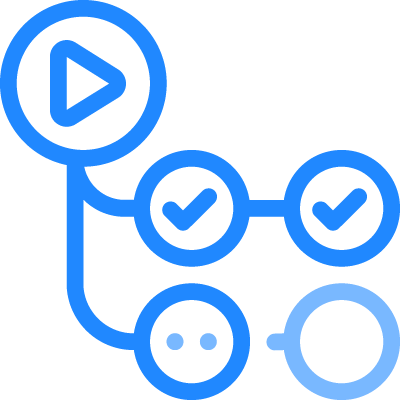
\includegraphics[width=\linewidth]{img/GithubActions-logo.png}
 \caption{Logotipo Github actions}\label{fig:LogoGithub}
\endminipage
\end{figure}

\begin{figure}[!htb]
   \minipage{0.19\textwidth}%
     
\includegraphics[width=\linewidth]{img/Quasar_logo.png}
     \caption{Logotipo Quasar}\label{fig:LogoQuasar}
     \endminipage\hfill
  \minipage{0.19\textwidth}%
    
\includegraphics[width=\linewidth]{img/apexcharts_logo.png}
    \caption{Logotipo Apexcharts}\label{fig:LogoApexcharts}
  \endminipage\hfill
  \minipage{0.19\textwidth}
   
\includegraphics[width=\linewidth]{img/Moby-logo.png}
   \caption{Logotipo Docker}\label{fig:LogoDocker}
  \endminipage\hfill
  \minipage{0.19\textwidth}
     
\includegraphics[width=\linewidth]{img/google_cloud_main.png}
     \caption{Logotipo Google Cloud}\label{fig:LogoGcloud}
  \endminipage\hfill
  \minipage{0.19\textwidth}%
     
\includegraphics[width=\linewidth]{img/logo-vmware.jpg}
     \caption{Logotipo Vmware}\label{fig:LogoVmware}
   \endminipage
\end{figure}

\chapter{Estudio de viabilidad. Método DAFO}

Esta aplicación estaría englobada dentro de las denominadas aplicaciones de productividad, con las aplicaciones de organización de horarios, calendarios y citas.

\section{Estudio de mercado}

Actualmente, si se realiza una búsqueda de aplicaciones de turnos, e incluimos en la búsqueda teletrabajo como palabra necesaria, no aparece ninguna aplicación. 

Sí hay aplicaciones de turnos, en los que se busca un control horario, pero actualmente prácticamente no hay ninguna aplicación centrada en el teletrabajo, en los turnos presenciales y no presenciales.

Hay controles horarios, que han aprovechado para incluir el teletrabajo dentro de la reclama de control horario, pero no gestionan los turnos.

Al ser una herramienta con un nicho tan específico, existe la posibilidad en la que el uso del teletrabajo vuelva a ser puramente testimonial, en la que la existencia de esta herramienta deje de ser necesaria.
\section{Análisis DAFO}
\begin{table} 
\begin{center}
\begin{tabular}{| c | c |}
\hline
Debilidades & Amenazas \\ \hline
\tiny Aplicación desconocida & \tiny Aparición de aplicaciones dedicadas \\
\tiny Programador con poco recorrido & \tiny Ampliación de aplicaciones actuales con esta opción \\
\tiny Uso puntual y específico & \tiny Disminución del teletrabajo\\
\tiny Falta de interés en la gestión de los turnos &  \\ \hline   
\normalsize
Fortalezas & Oportunidades \\ \hline
\tiny Posibilidad de personalización de forma sencilla & \tiny Mercado prácticamente exclusivo \\
\tiny Sencillez de uso &  \tiny Fácil de integrar en otras webs\\
\tiny Despliegue sencillo & \tiny El teletrabajo está de moda \\
\hline
\end{tabular}
\caption{Matriz DAFO}
\label{table:1}
\end{center}
\end{table}
\section{Planificación temporal}
Para la planificación temporal tendremos en cuenta como fecha de inicio la primera semana de marzo, y como fecha final la semana del 17 al 23 de mayo.
Tendremos como margen 1 o 2 semanas para resolver cualquier desviación sobre la planificación inicial.

El ritmo de trabajo será de entre 2 o 3 horas diarias, incrementándose hasta unas posibles 5 o 6 horas los fines de semana. 

\begin{figure}[h!] % [h!]
   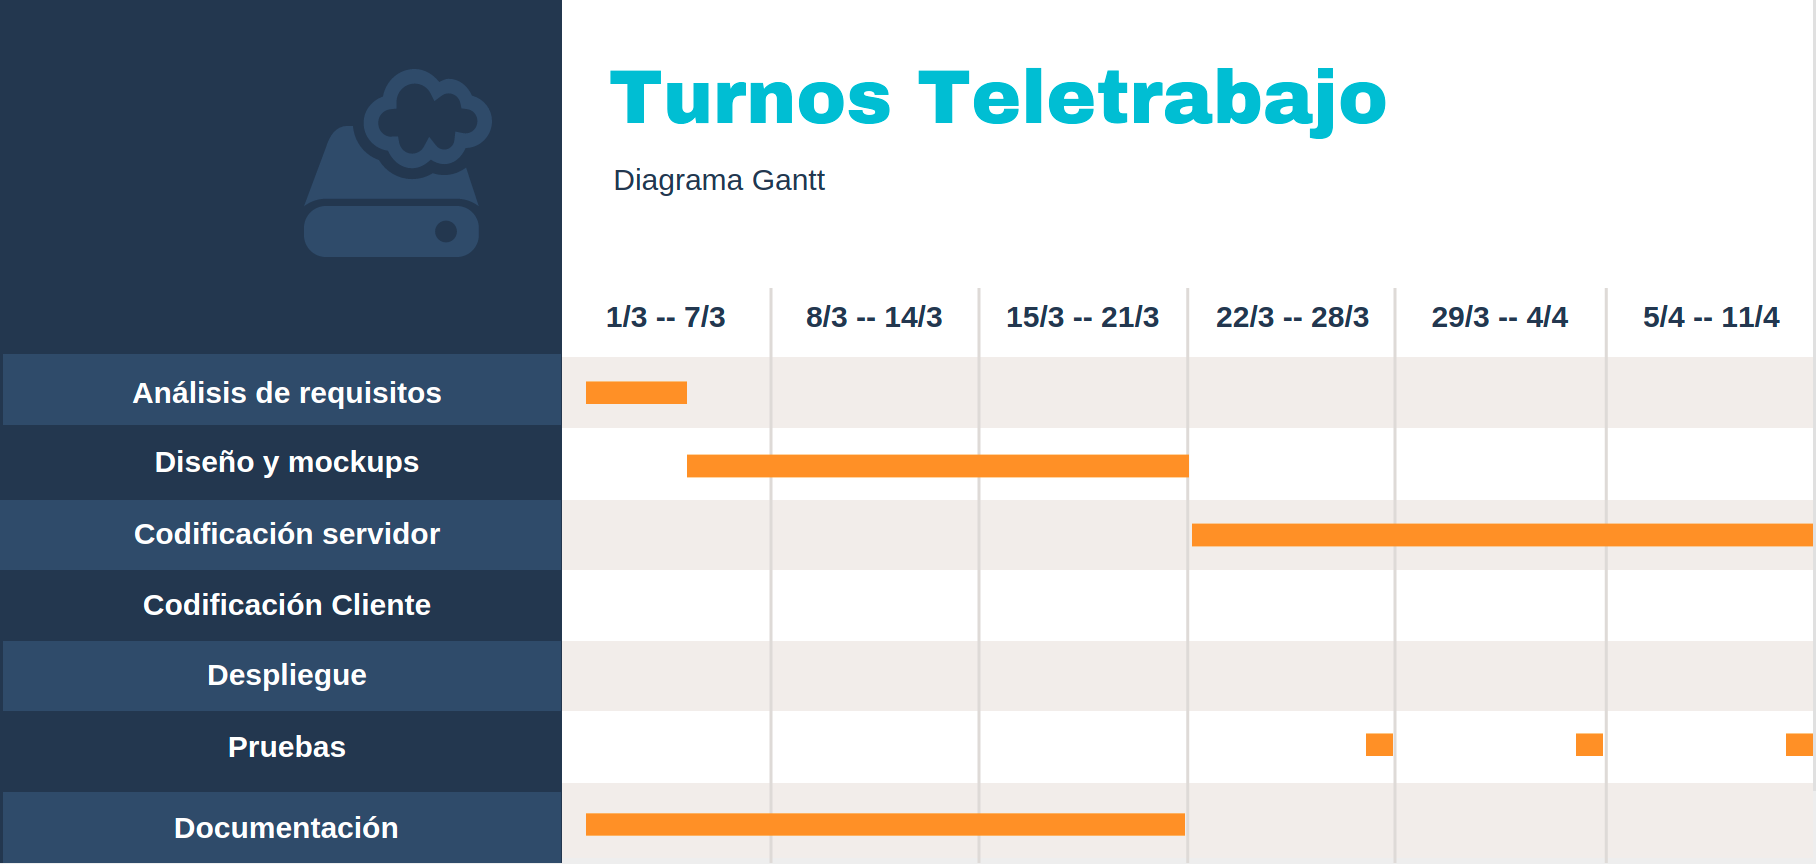
\includegraphics[width=\linewidth]{img/gantt1.png}
   \caption{Primer segmento Gantt}
   \label{fig:Gantt1}
 \end{figure}

 \begin{figure}[h!] % [h!]
   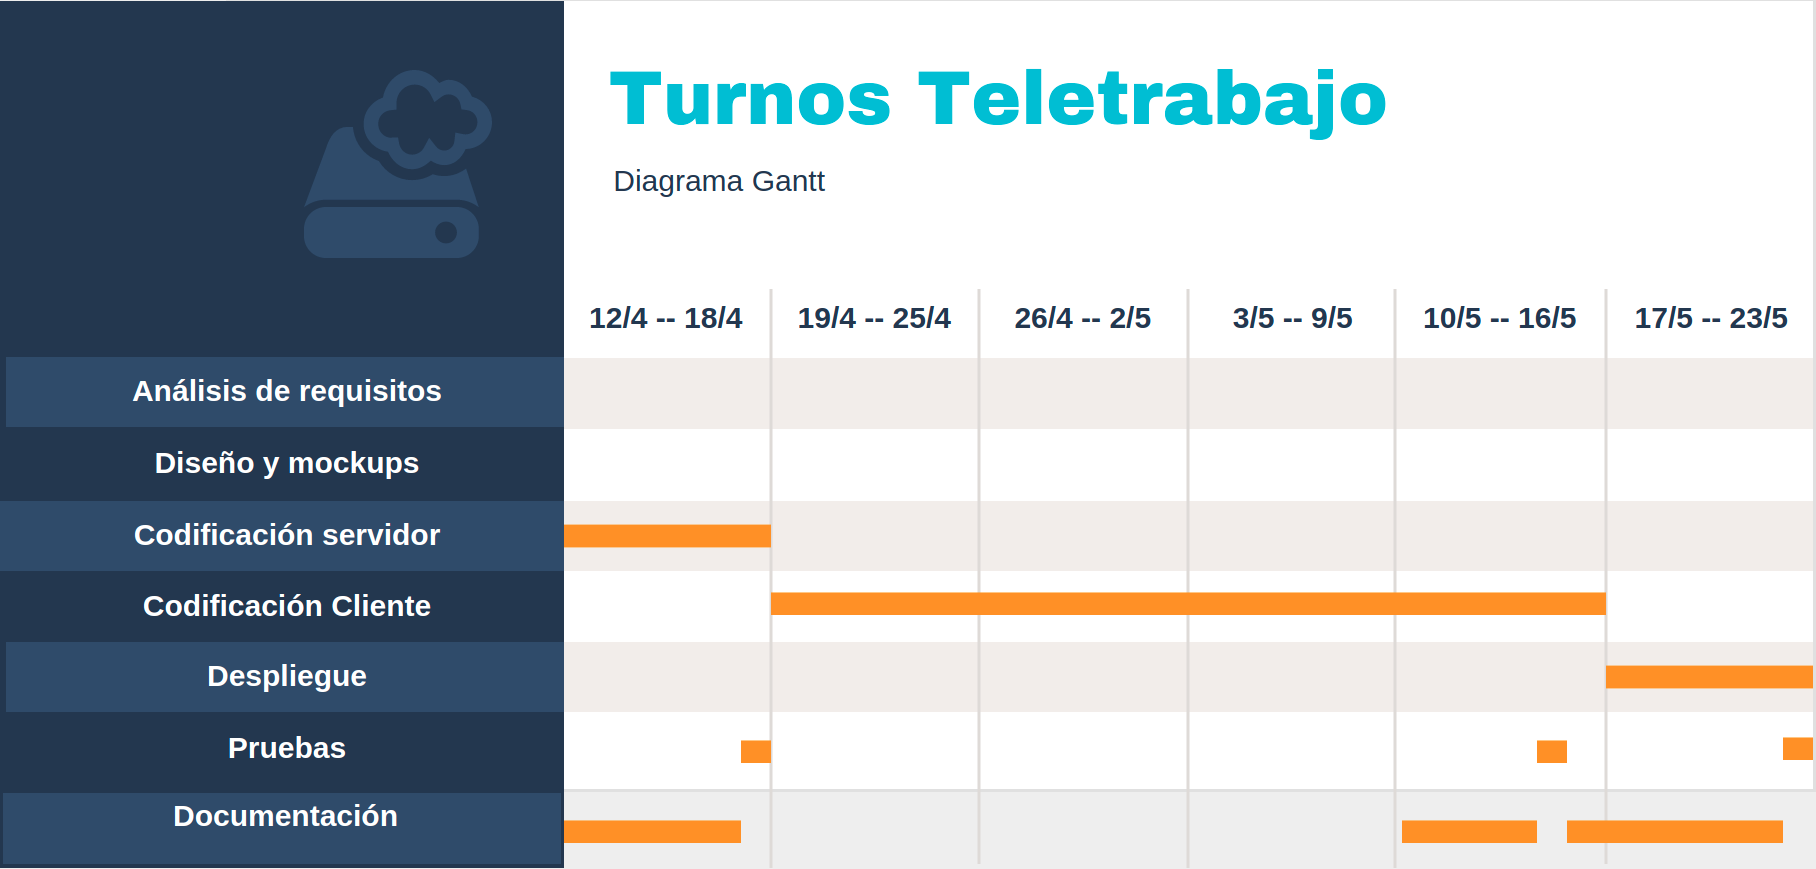
\includegraphics[width=\linewidth]{img/gantt2.png}
   \caption{Segundo segmento Gantt}
   \label{fig:Gantt21}
 \end{figure}
 \pagebreak
\begin{itemize}
   \item Análisis de requisitos  (3 días)  
   \item Diseño y mockups (18 días)
   \begin{itemize}
      \item Diseño arquitectura
      \item Mockups
      \item Diagrama de componentes
      \item Diagrama mysql
      \item Mapa web
   \end{itemize}
   \item Codificación entorno servidor (28 días)
   \begin{itemize}
      \item Creación modelos sequelize
      \item Implementar autenticación
      \item Creación de rutas
      \item Pruebas de funcionamiento (Postman)
   \end{itemize}
   \item Codificación entorno cliente (28 días)
   \begin{itemize}
      \item Autenticación
      \item Calendario
      \item Personalización
      \item Informes
      \item Panel administrador
      \item Pruebas de funcionamiento
   \end{itemize}
   \item Despliegue (7 días)
   \begin{itemize}
      \item Creación de contenedores
      \item Despliegue servidor dedicado
      \item Despliegue Google Cloud
      \item Pruebas de funcionamiento
   \end{itemize}
   \item Documentación (40 días a lo largo del proyecto)
\end{itemize}

\chapter{Análisis de requisitos}

La aplicación es para gestionar los días en los que se va a teletrabajar y los días en los que se realizará el turno presencial. 
Por lo tanto, es necesario ver una representación de los días de la semana, y los días en los que se trabajará presencialmente (o los que no).

Dependiendo quien acceda, tendrá unos privilegios para realizar cambios en su calendario, en el de otros, obtener informes, o cambiar la configuración de toda la aplicación, por lo que se debe identificar a la persona que entra y comprobar su nivel de acceso a la aplicación.

Un trabajador, con el acceso más básico, debería ser capaz de hacer las siguientes acciones:

\begin{itemize}
   \item Ver los días que le toca trabajar de forma presencial.
   \item Ver los días que ha trabajado de forma presencial.
   \item Ver quien irá de forma presencial de su área.
   \item Confirmar los días que le han sido asignados.
   \item Solicitar un cambio de día presencial.
\end{itemize}

Un responsable de departamento, aparte del acceso básico, debería ser capaz de:

\begin{itemize}
   \item Modificar el calendario de los trabajadores de su departamento.
   \item Ver el calendario global.
   \item Validar o rechazar la petición de cambios.
   \item Generar un informe de su departamento.
\end{itemize}

Y el responsable o administrador de la aplicación, aparte de todas las funciones anteriores, debe ser capaz de:

\begin{itemize}
   \item Modificar todo el calendario.
   \item Modificar los parámetros de la aplicación.
   \item Crear y asignar usuarios a departamentos.
   \item Generar un informe completo.
\end{itemize}

Los trabajadores deberían ser capaces de personalizar su perfil, con colores, iconos, fotografía, etc.

\section{Diagrama de casos de uso}

Se ha realizado un diagrama de casos de uso, donde mostramos una vez autenticado el trabajador, qué acciones puede realizar.

\begin{figure}[h!] % [h!]
   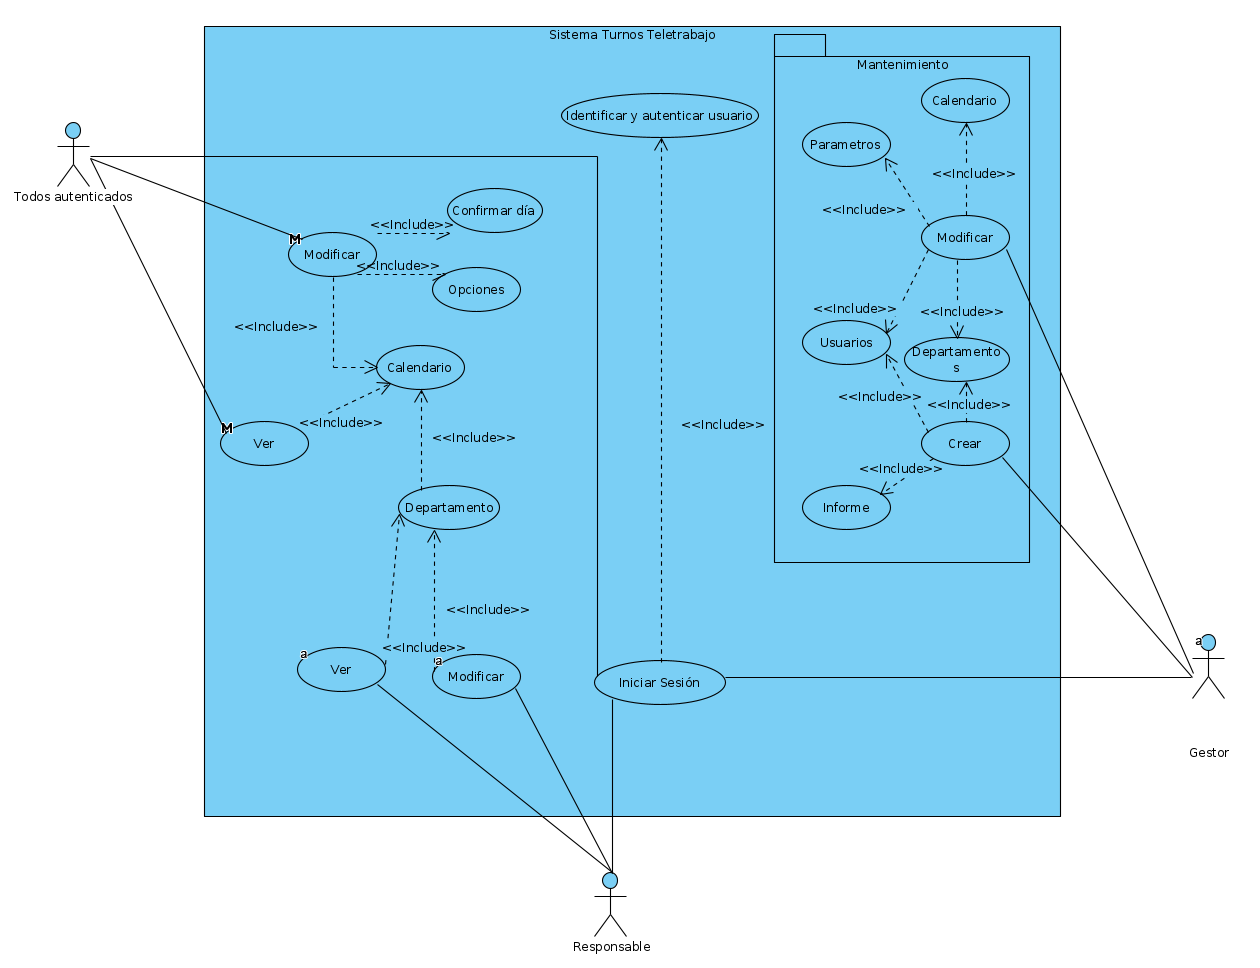
\includegraphics[width=\linewidth]{img/Casos de uso.png}
   \caption{Diagrama de casos de uso}
   \label{fig:CasosUso1}
 \end{figure}

\chapter{Diseño}

\section{Diseño Conceptual Entidad Relación}
A partir del análisis de los requisitos, se obtiene el siguiente diseño conceptual E/R.

\begin{figure}[h!] % [h!]
  \centering
   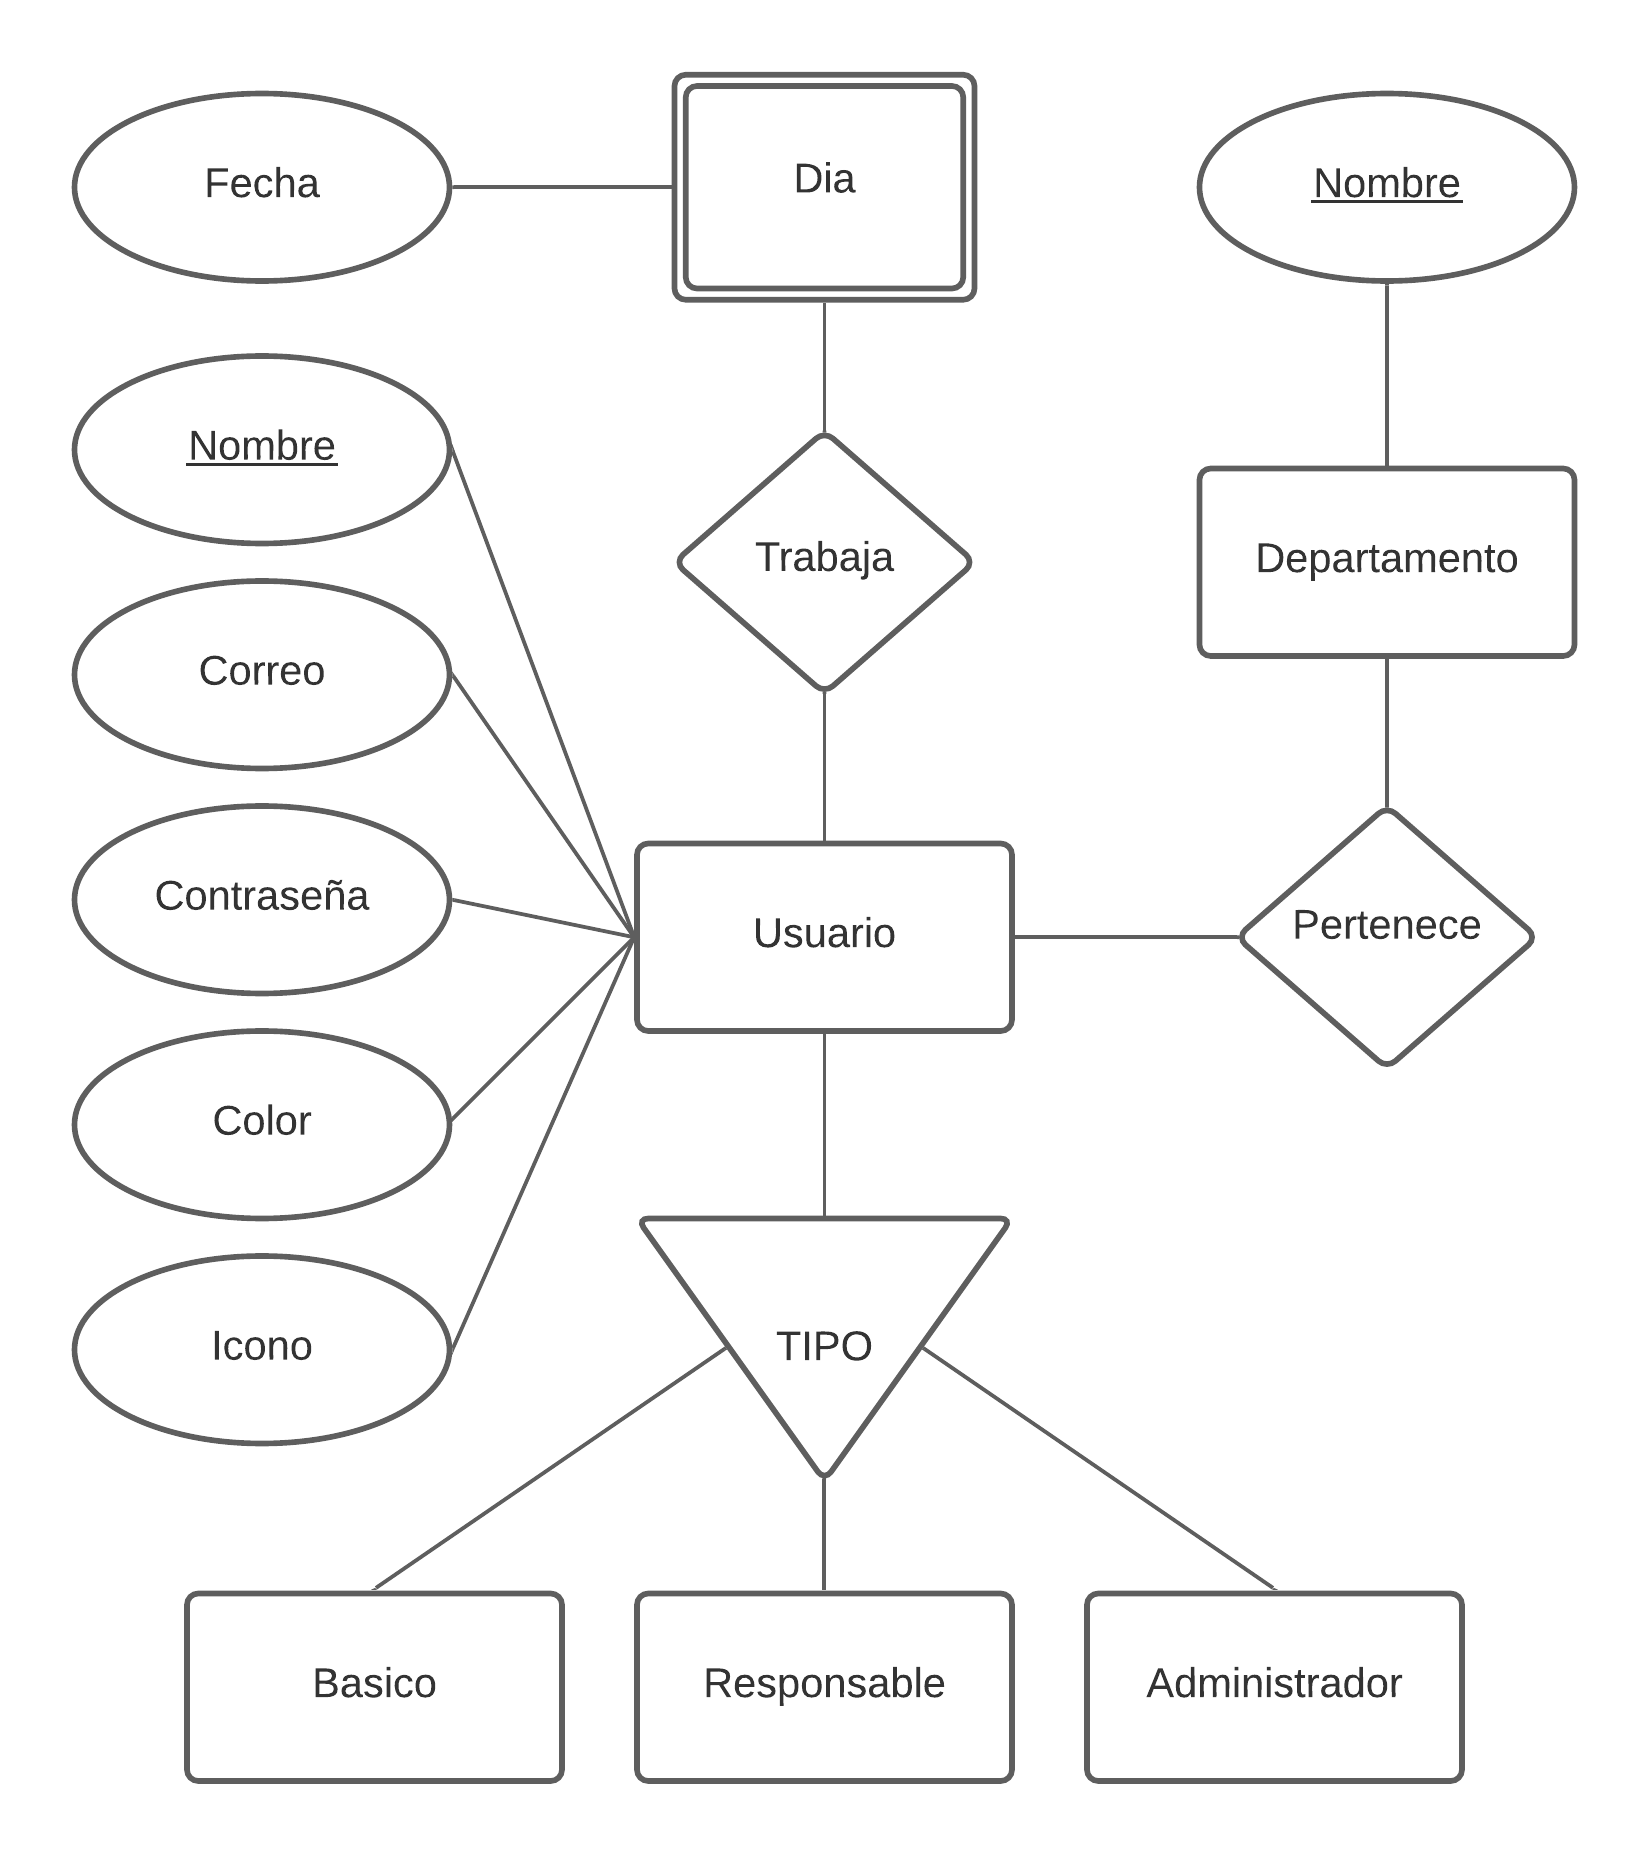
\includegraphics[scale=0.45]{img/EntidadRelacion.png}
   \caption{Diagrama E/R}
   \label{fig:diagramaer}
 \end{figure}

 Finalmente, se ha cambiado el diseño de forma que Tipo y Departamento son atributos de Usuario, creando una única relación entre el usuario y los días que trabaja de forma presencial.
 \begin{figure}[h!] % [h!]
  \centering
   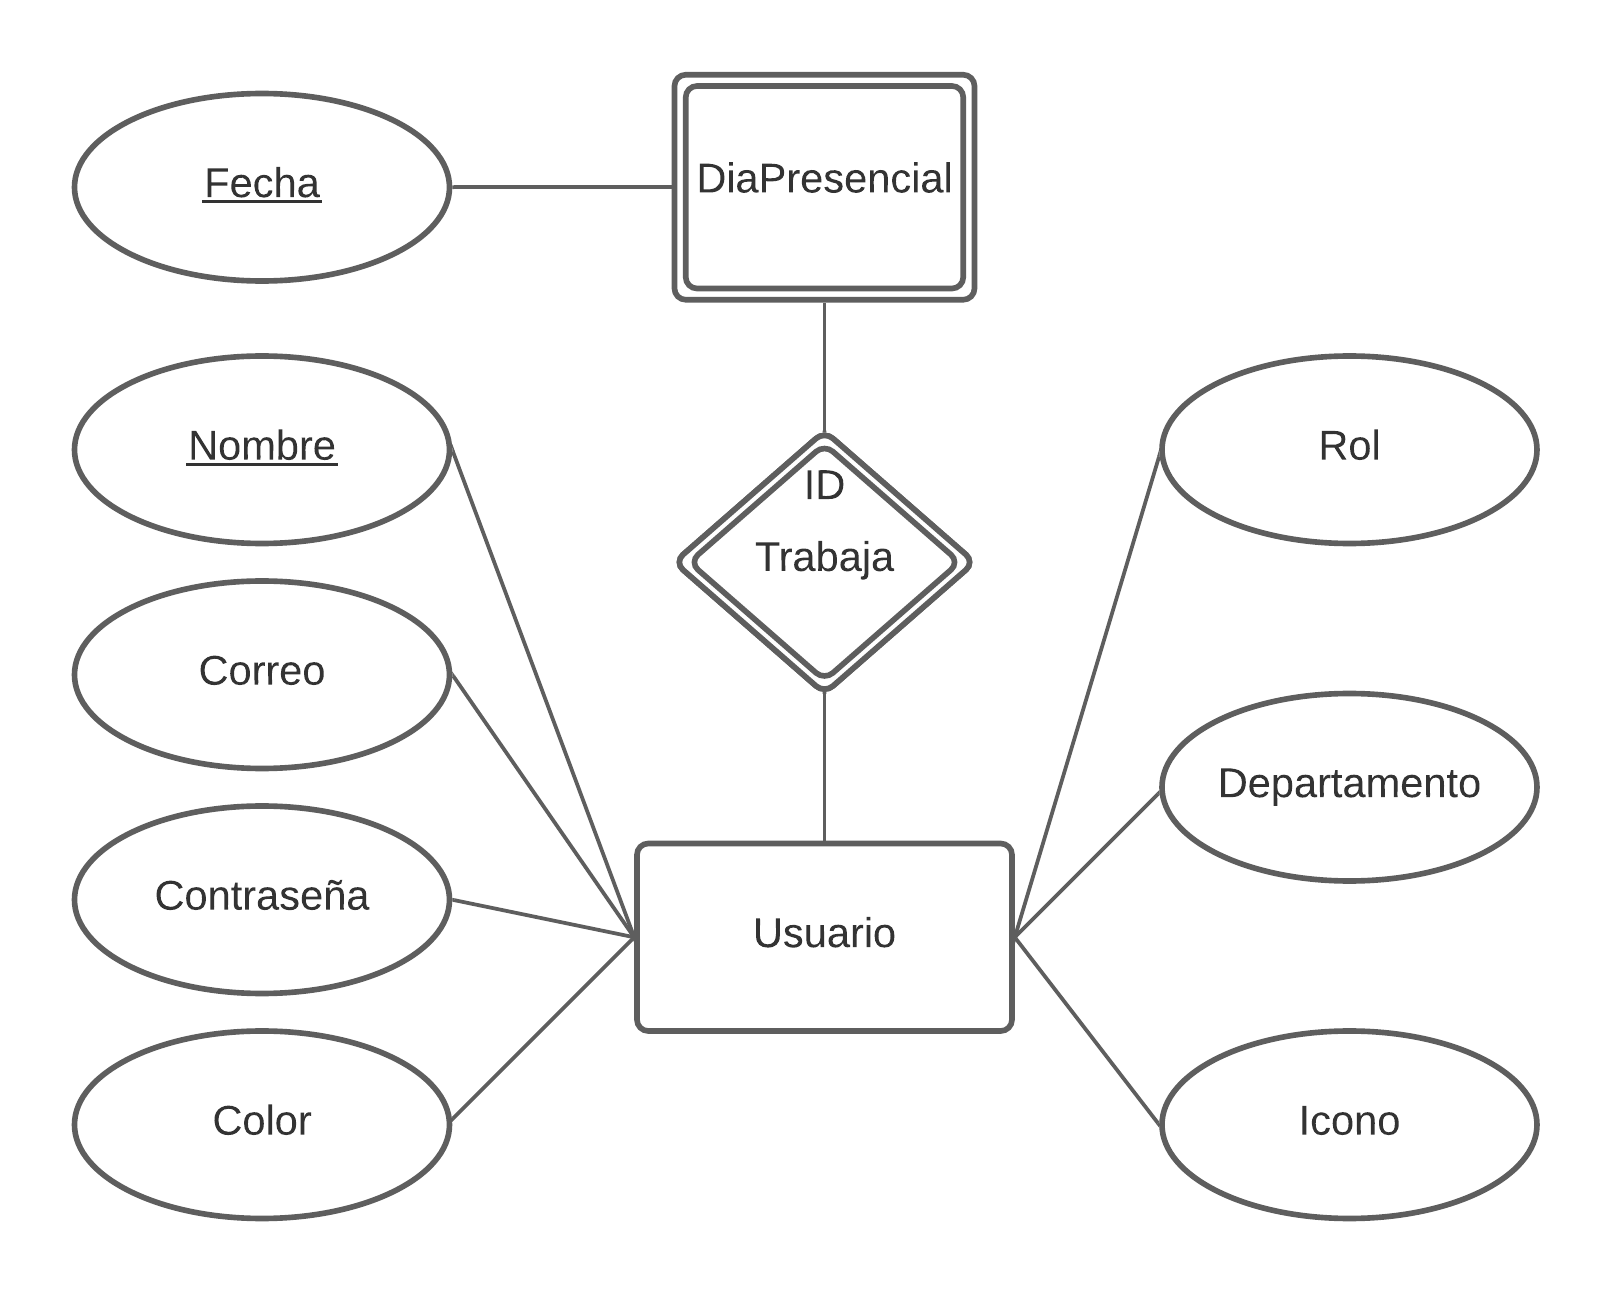
\includegraphics[scale=0.45]{img/DiagramaERFinal.png}
   \caption{Diagrama E/R}
   \label{fig:diagramaerfinal}
 \end{figure}


\section{Diseño Lógico Relacional o Paso a tablas}
Siguiendo el esquema E/R inicial, el paso a tablas de las entidades y relaciones sería el siguiente:

\begin{figure}[h!] % [h!]
  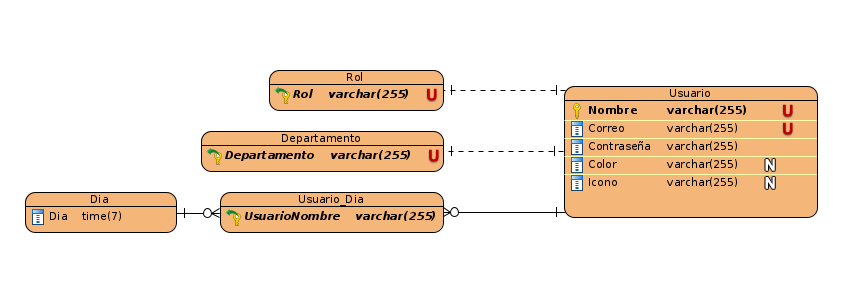
\includegraphics[width=\linewidth]{img/pasotablas.png}
  \caption{Diagrama Lógico Relacional}
  \label{fig:diagramalr}
\end{figure}

Con la simplificación, el diseño quedaría de la siguiente forma:

\begin{figure}[h!] % [h!]
  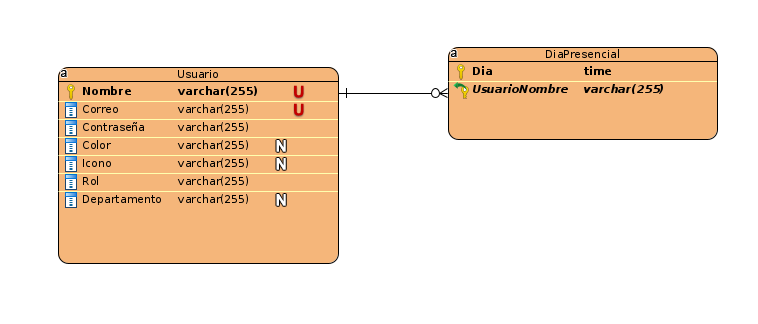
\includegraphics[width=\linewidth]{img/DiagramaBBDDfinal.png}
  \caption{Diagrama Lógico Relacional final}
  \label{fig:diagramalrfinal}
\end{figure}

Este no ha sido el diseño definitivo, puesto que por, sencillez de trabajo, se ha decidido asignar una clave primaria distinta a la que sale naturalmente.
\clearpage

\section{Diseño Físico o Diagrama Mysql}
En el diseño físico se ha incluido funcionalidad de sequelize, que permite automatizar la fecha de creación y modificación de los campos.
También se ha añadido como clave primaria un id en todas las tablas, para trabajar de forma más cómoda en la API.
Por último, se ha aprovechado también la auto creación de relaciones entre tablas, para que nombrase automáticamente las relaciones.

Según el esquema inicial, el diagrama mysql hubiera sido el siguiente:
\begin{figure}[h!] % [h!]
  \centering
   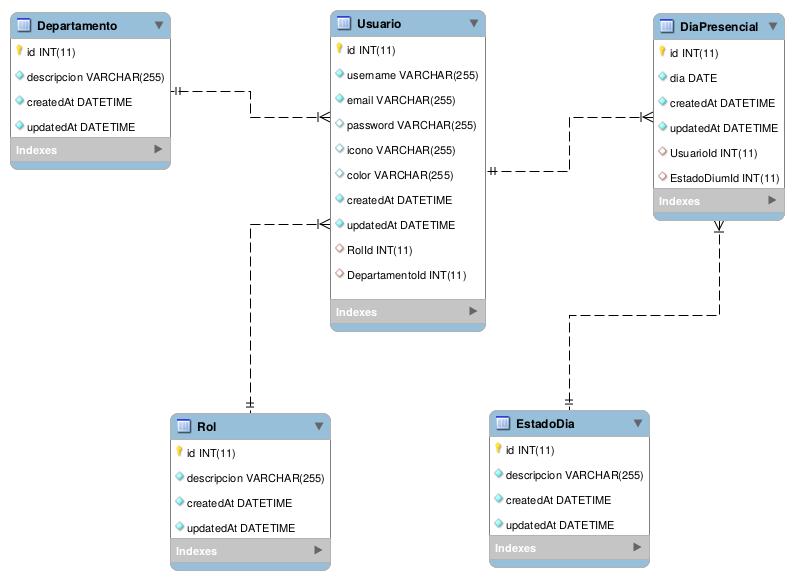
\includegraphics[scale=0.40]{img/EsquemaBBDD.png}
   \caption{Diagrama mysql}
   \label{fig:diagramaMysql}
 \end{figure}

 Al simplificar la base de datos, y creando una clave primaria numérica id, finalmente se obtiene el siguiente esquema, en el que sólo hay 2 tablas, que se relacionan mediante el id de usuario. 
 \begin{figure}[h!] % [h!]
  \centering
  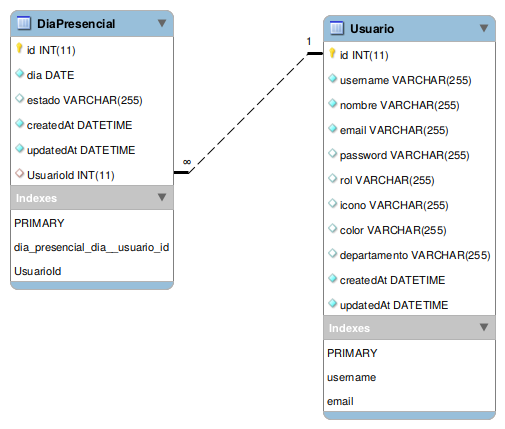
\includegraphics[scale=0.40]{img/nuevaBBDD.png}
  \caption{Diagrama mysql final}
  \label{fig:nuevodiagramaMysql}
\end{figure}
\clearpage 

\section{Mockups}

\begin{figure}[ht!] % [h!]
   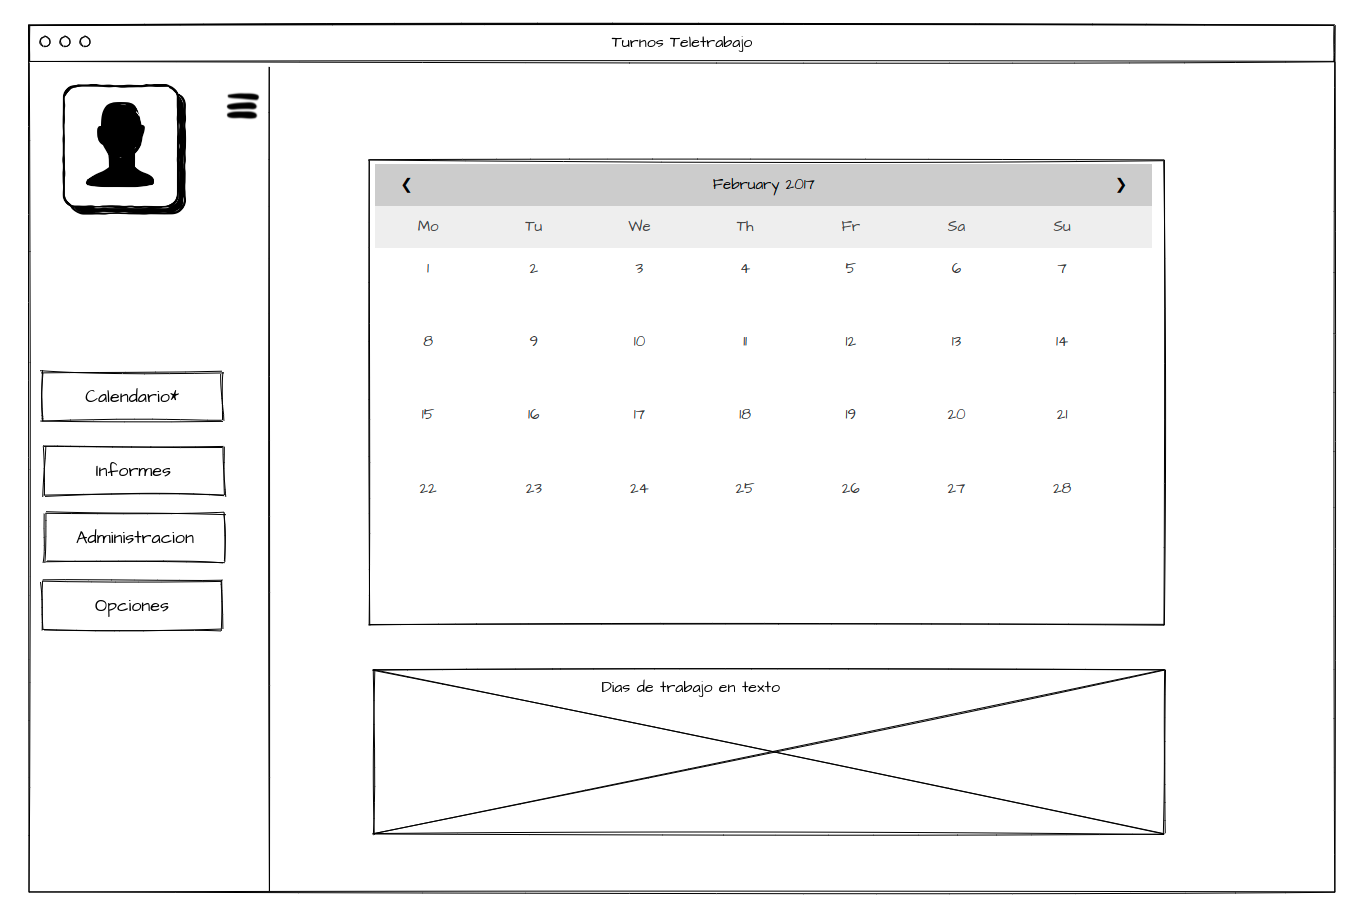
\includegraphics[width=0.48\textwidth]{img/Vista_Calendario_PC.png}
   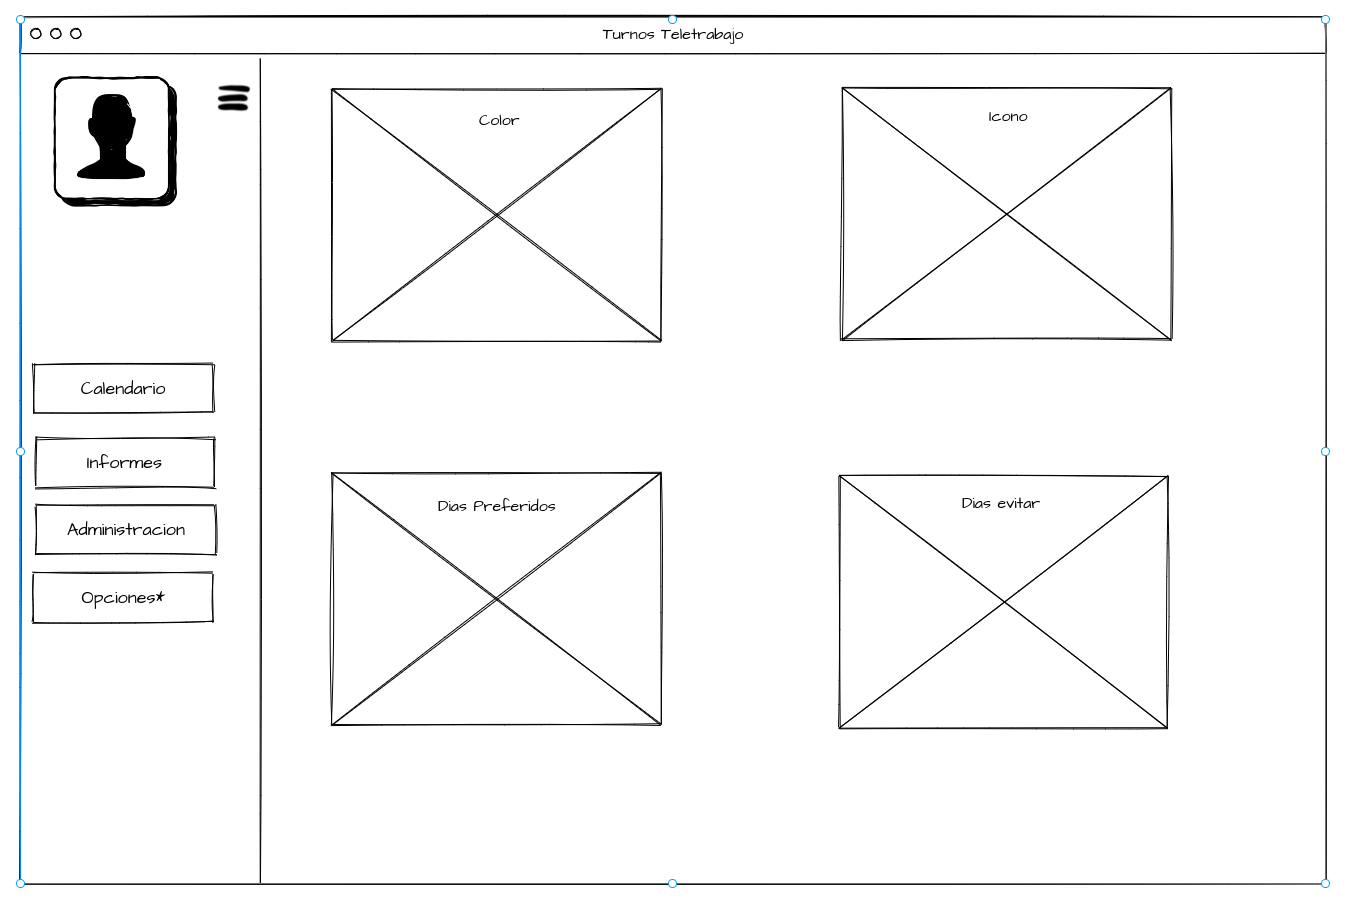
\includegraphics[width=0.48\textwidth]{img/Vista_Opciones_PC.png}
   \caption{Mockup vista calendario y opciones versión pc}
   \label{fig:calendarioPC}
 \end{figure}

 \begin{figure}[ht!] % [h!]
   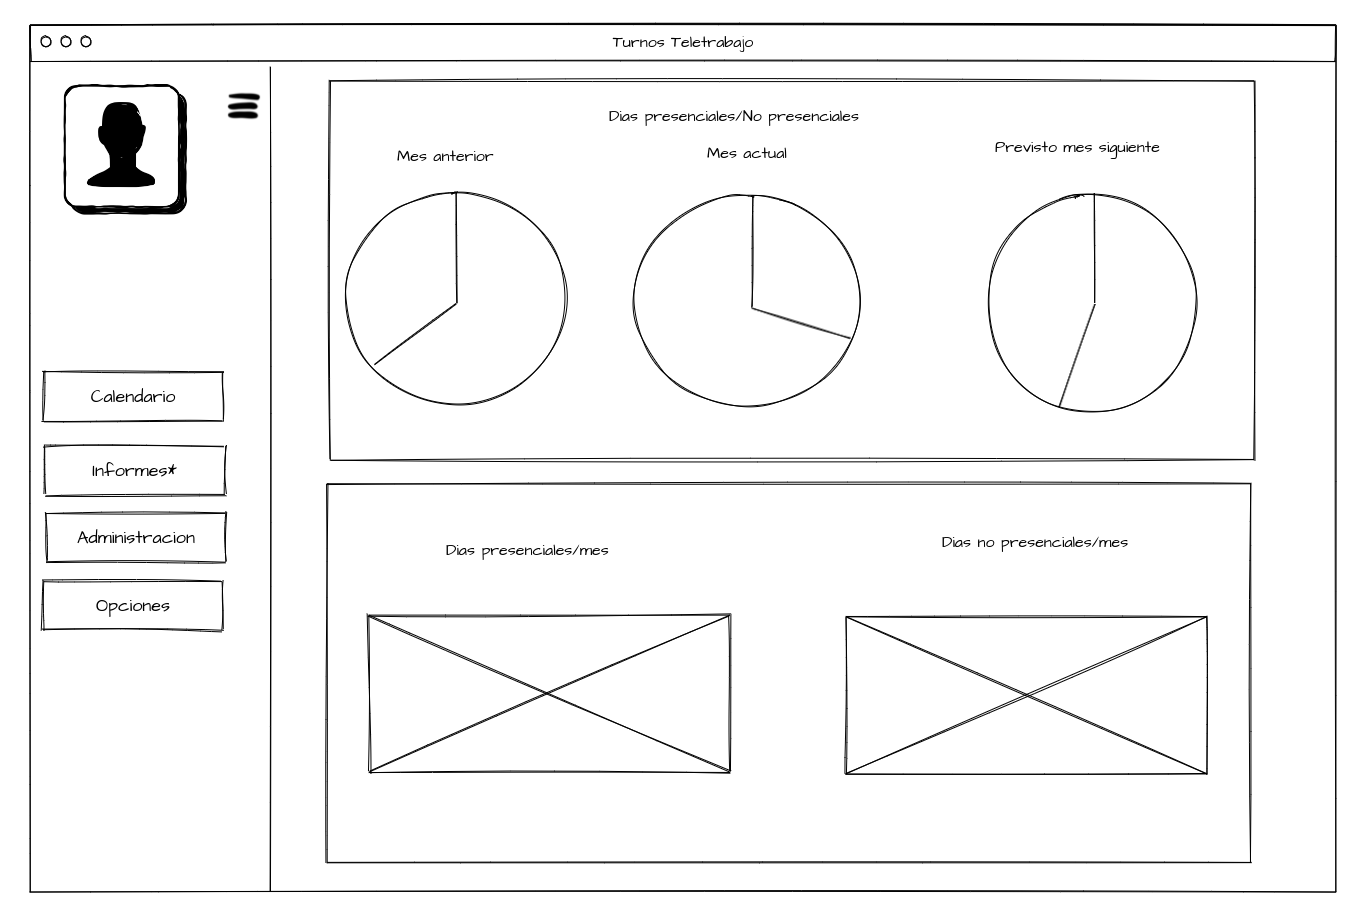
\includegraphics[width=0.48\textwidth]{img/Vista_Informes_PC.png}
   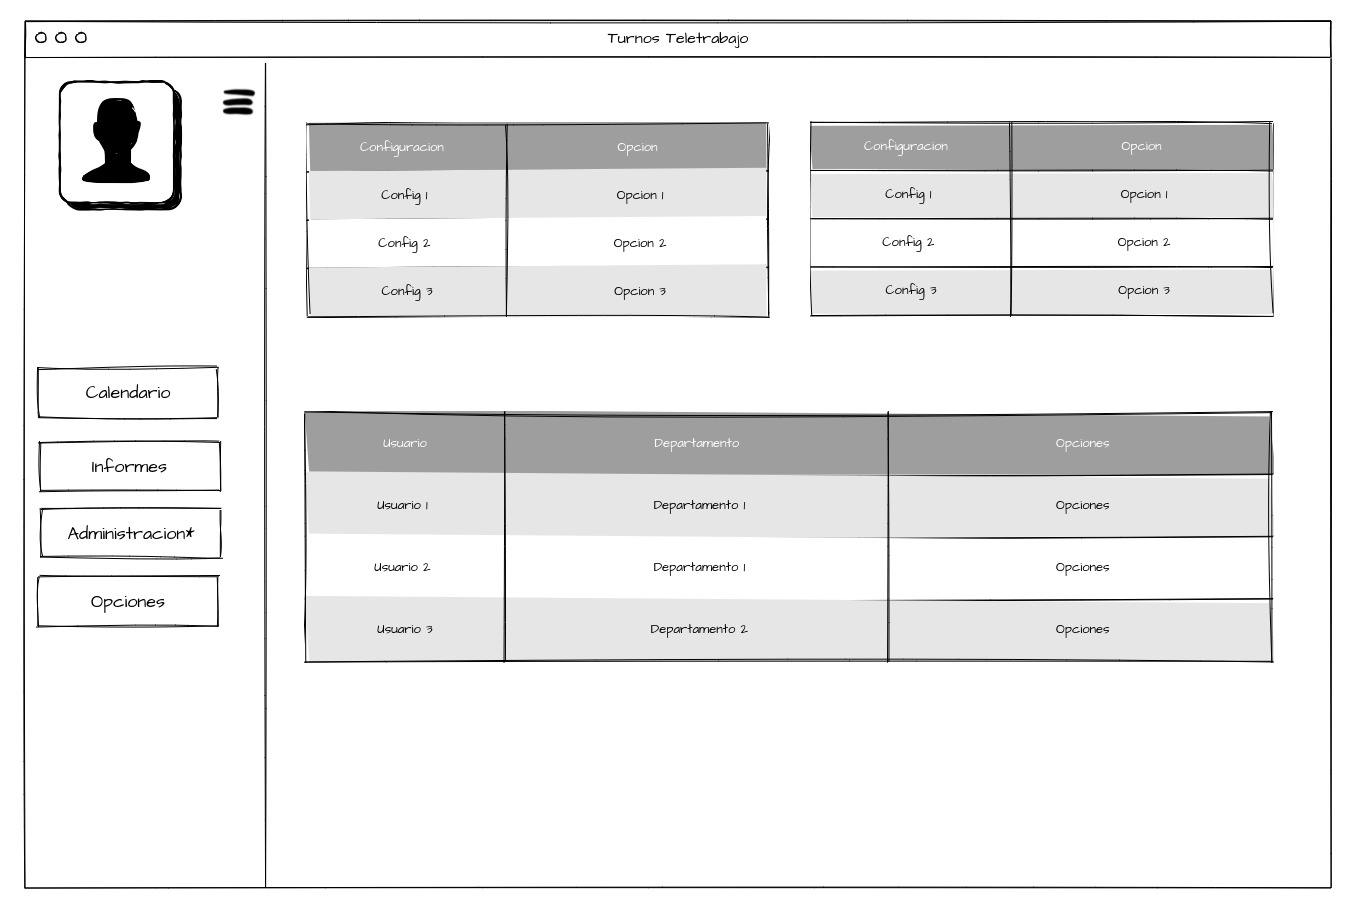
\includegraphics[width=0.48\textwidth]{img/Vista_Administracion_PC.png}
   \caption{Mockup vista informes y administración versión pc}
   \label{fig:informesPC}
 \end{figure}

 \begin{figure}[ht!] % [h!]
  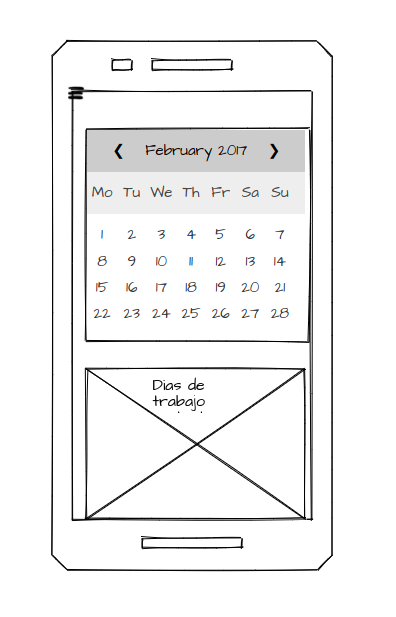
\includegraphics[width=0.24\textwidth]{img/Vista_Calendario_MVL.png}
  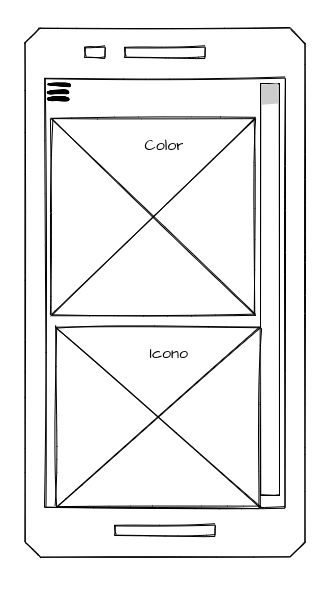
\includegraphics[width=0.24\textwidth]{img/Vista_Opciones_MVL.png}
  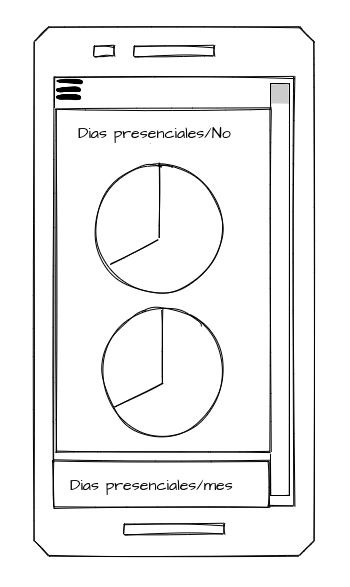
\includegraphics[width=0.24\textwidth]{img/Vista_Informes_MVL.png}
  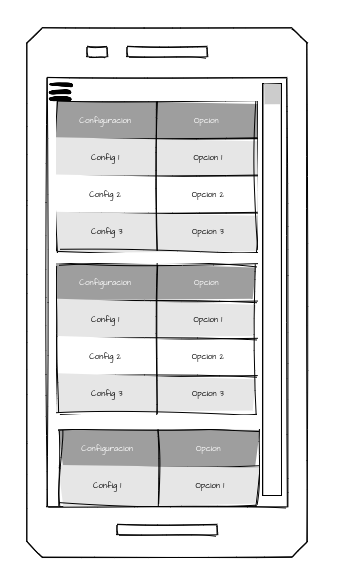
\includegraphics[width=0.24\textwidth]{img/Vista_Administracion_MVL.png}
  \caption{Mockup móvil}
  \label{fig:VistaMVL}
\end{figure}

\chapter{Codificación}

\section{Tecnologías elegidas y su justificación}

Se ha usado \LaTeX{} para crear la documentación, que está formado por un gran conjunto de macros de TeX, siendo un lenguaje de marcas. 
Se Ha elegido \LaTeX{} frente a Word o LibreOffice, ya que se conocía el lenguaje con anterioridad, \LaTeX{} permite automáticamente colorear el código, y la presentación parece más profesional.

\begin{figure}[ht!] % [h!]
  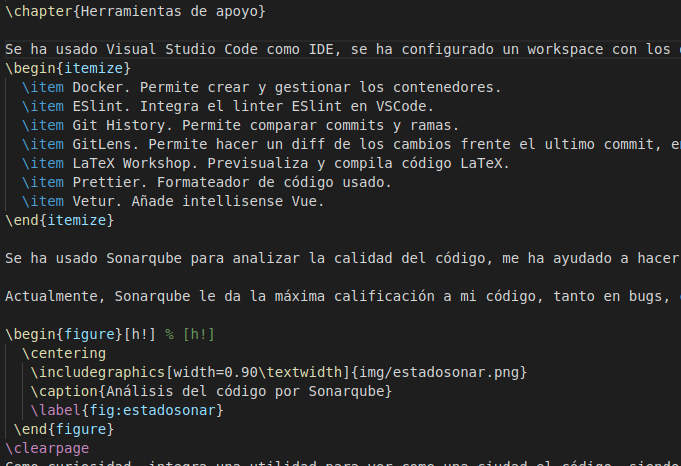
\includegraphics[width=0.54\textwidth]{img/LatexCode2.png}
  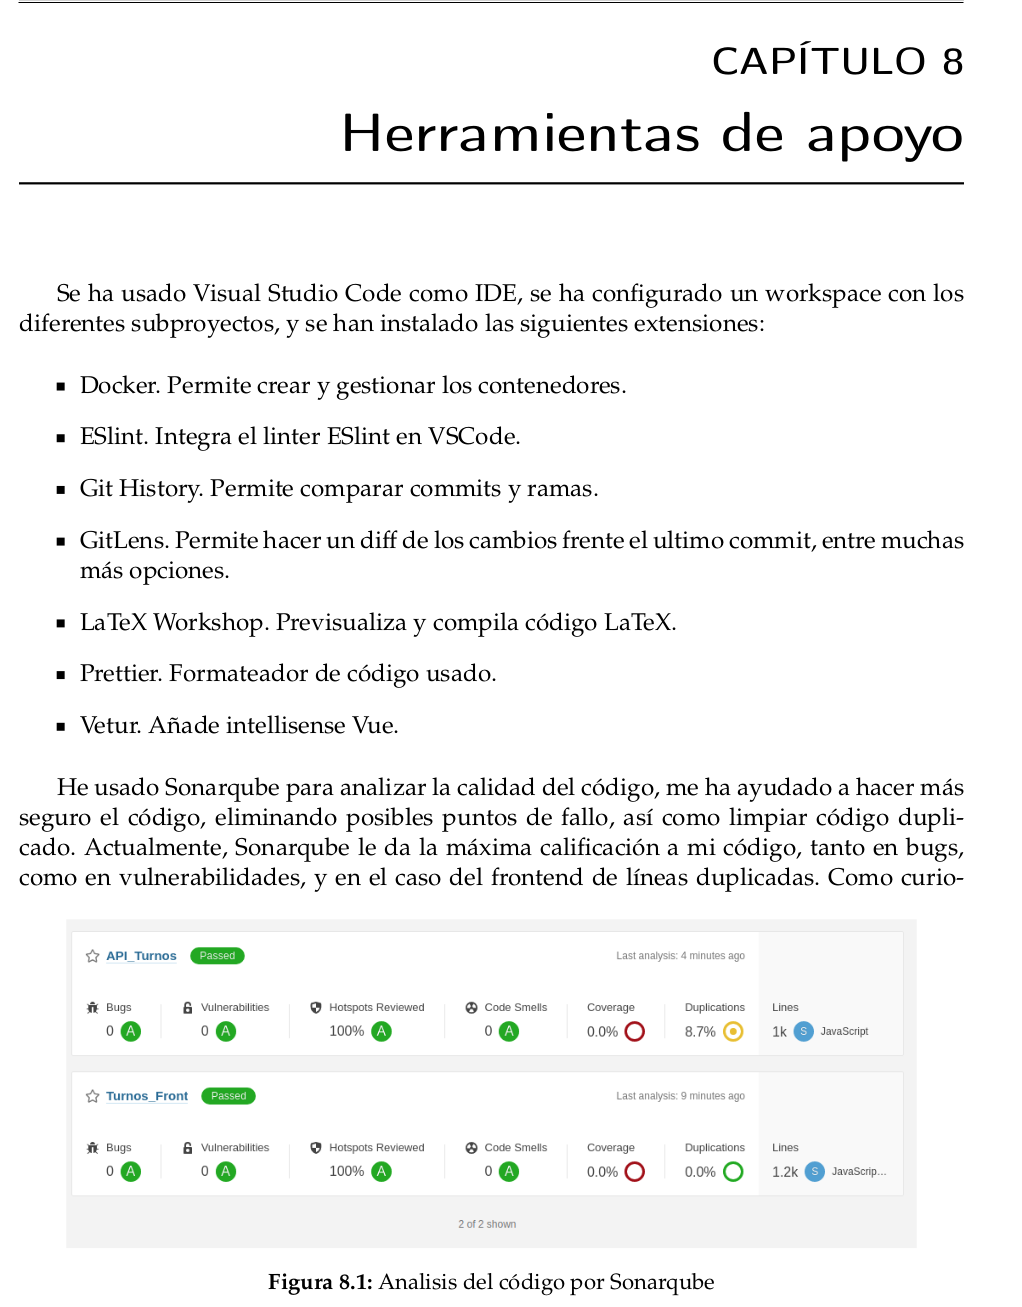
\includegraphics[width=0.44\textwidth]{img/LatexCompilado.png}
  \caption{Código fuente VS salida compilada}
  \label{fig:Latex}
\end{figure}

Se ha programado en JavaScript tanto el frontend como el backend, facilitando tanto el mantenimiento como el desarrollo al unificar la programación en un único lenguaje.

En backend se ha usado la combinación de Node.js como motor de ejecución de javascript y Express como framework web, siendo una combinación muy usada para crear REST API.

Para el acceso a la base de datos se ha optado por usar el ORM Sequelize, que conjuntamente con el uso de las promesas de javascript dota de funcionamiento ininterrumpido el backend. 
También realiza la función de prevenir la inyección de sql, si bien es cierto que en Sequelize 3.x y 5.x se descubrieron unas vulnerabilidades que permitían inyectar código sql en mariadb, se parchearon de forma definitiva en la versión 5.15.1, en el proyecto se ha usado la versión 6.6.2

Para la gestión de accesos y contraseñas se ha usado el paquete node jsonwebtoken (JWT), que es componente de uso común para gestionar las sesiones entre cliente y servidor, y para encriptar la contraseña se ha usado el módulo bcrypt.

En el frontend se ha usado Quasar, para poder generar una aplicación móvil e instalarla a través de herramientas MDM como SOTI, una aplicación de escritorio para los sistemas cerrados en los que no hay instalado un navegador, y la aplicación web de acceso común para el resto del personal.
Se ha usado la librería QCalendar de Quasar, que dota de funciones de fecha/hora, así como un interfaz de calendario mensual, semanal y diario, siendo así innecesario tener que crear todo el calendario desde cero.

Para el acceso a la api, se ha usado axios, que es el módulo que recomienda Quasar para las peticiones Ajax. Se ha usado Vuex para almacenar el estado de la autenticación.
En la personalización de los usuarios adopté el módulo qiconpicker para elegir el icono personal y vue-html2pdf para imprimir el calendario. Vue-html2pdf es un componente basado en html2pdf, que te permite elegir el componente vue a imprimir directamente, su funcionalidad prácticamente es la misma que html2pdf.

Se han usado imágenes docker compatibles tanto con windows como con linux. Para esto se ha tenido que realizar algún sacrificio, como no usar el cron de linux, pero la aplicación completa puede correr en ambos sistemas. Posiblemente funcione en macOS, pero no ha sido posible probarlo.
Se puede usar tanto el docker-compose suministrado como levantar los distintos contenedores en equipos distintos, sólo necesario configurar el fichero de cliente, así se puede desplegar prácticamente sin esfuerzo, a través de los contenedores ya creados desde dockerhub , o creándolos a través de sus fuentes de github. 

Se ha usado yaml para el fichero de configuración de docker-compose y las acciones de github, no se ha podido elegir json ni otras alternativas, al ser el formato elegido por docker y github. 

\section{Entorno servidor}
El código fuente del frontend está alojado en github en la siguiente dirección: \\
\url{https://github.com/jrinconm/TurnosApi}

Node.js es un motor de ejecución JavaScript muy ligero, que puede realizar funciones de servidor web. 
En niveles de carga altos, su rendimiento está por debajo de nginx o apache, pero para las necesidades que tenemos para la API, es rendimiento suficiente y funciona de forma correcta.

Gracias al middleware Express, se ha creado una API de forma simple, dividiendo las rutas en ficheros para modularizar la aplicación, así si hay que modificar algún punto, no es necesario modificar toda la aplicación, sólo el fichero de la ruta.

\begin{lstlisting}[style=ES6, caption={Importación rutas para Express}]
  require("./app/routes/departamento.routes")(app);
  require("./app/routes/diapresencial.routes")(app);
  require("./app/routes/estadodia.routes")(app);
  require("./app/routes/rol.routes")(app);
  require("./app/routes/user.routes")(app);
  require("./app/routes/auth.routes")(app);
\end{lstlisting}

  En caso de querer cambiar el puerto, sólo hay que modificar el fichero server.js, para cambiar la constante PORT por el puerto que queramos usar. 

\begin{lstlisting}[style=ES6, caption={Configuración del puerto de la API }]
  // set port, listen for requests
  const PORT = process.env.PORT || 8080;
  app.listen(PORT, () => {
  console.log(`Server is running on port ${PORT}.`);
  });
\end{lstlisting}

Sequelize es uno de los ORM más usados en JavaScript, securizando el acceso a los datos. 
La configuración se realiza a través de un objeto en el fichero config/db.config.js, la contraseña debe ser la misma que la que se ha configurado en la base de datos.
A continuación un ejemplo de la configuración de la base de datos, con una contraseña a modo de ejemplo.

\begin{lstlisting}[style=ES6, caption={Configuración de la BBDD para Sequelize}]
  module.exports = {
    HOST: "mariadb",
    USER: "root",
    PASSWORD: "qwerty",
    DB: "TurnosTeletrabajo",
    dialect: "mysql",
    pool: {
      max: 5,
      min: 0,
      acquire: 30000,
      idle: 10000,
    },
  };
\end{lstlisting}
Este objeto se importa al inicializar Sequelize:
\begin{lstlisting}[style=ES6, caption={Importación de la configuración e instanciación de Sequelize}]
  const config = require("../config/db.config.js");
  const Sequelize = require("sequelize");
  const sequelize = new Sequelize(config.DB, config.USER, config.PASSWORD, {
    host: config.HOST,
    dialect: config.dialect,
    pool: {
      max: config.pool.max,
      min: config.pool.min,
      acquire: config.pool.acquire,
      idle: config.pool.idle,
    },
  });
\end{lstlisting}

La mayoría de la documentación existente en Internet no usa sus clases, sino que directamente crea objetos. 

En esta aplicación hemos usado las clases existentes para poder eliminar código duplicado existente en la creación de todos los objetos.
En el caso de querer modificar algo, por ejemplo, eliminar el id para que el propio nombre fuera la clave principal, sólo tendría que modificar la clase base, no todos los objetos.

Objetos Sequelize:

\begin{lstlisting}[style=ES6, caption={Objeto Departamento}]
module.exports = (sequelize, Sequelize) => {
  const Departamento = sequelize.define(
    "departamento",
    {
      id_departamento: {
        type: Sequelize.INTEGER,
        autoIncrement: true,
        primaryKey: true,
      },
      departamento: {  
        type: Sequelize.STRING 
        },
    },
    { 
      // Elimino el cambio de nombre en la tabla
      freezeTableName: true 
      }
  );

  return Departamento;
};
\end{lstlisting}


\begin{lstlisting}[style=ES6, caption={Objeto Rol}]
module.exports = (sequelize, Sequelize) => {
  const Rol = sequelize.define(
    "rol",
    {
      id_rol: {
        type: Sequelize.INTEGER,
        autoIncrement: true,
        primaryKey: true,
      },
      rol: {
        type: Sequelize.STRING,
      },
    },
    {
      // Elimino el cambio de nombre en la tabla
      freezeTableName: true,
    }
  );

  return Rol;
};
\end{lstlisting}
\clearpage

Clases Sequelize (a la clase base se le ha añadido un getter):

\begin{lstlisting}[style=ES6, caption={Clase base}]
  const Sequelize = require("sequelize");
  class baseIdNombre extends Sequelize.Model {
    static init(sequelize) {
      return super.init(
        {
          id: {
            type: Sequelize.INTEGER,
            autoIncrement: true,
            primaryKey: true,
          },
          descripcion: {
            type: Sequelize.STRING,
            allowNull: false,
            unique: true,
          },
        },
        {          
          freezeTableName: true,
          sequelize,
        }
      );
    }
    static getId(where) {
      return this.findOne({
        where, attributes: ["id"],
        order: [["createdAt", "DESC"]],
      });
    }
    static getDesc(where) {
      return this.findOne({
        where, attributes: ["descripcion"],
        order: [["createdAt", "DESC"]],
      });
    }
  }
  module.exports = baseIdNombre;
\end{lstlisting}

\begin{lstlisting}[style=ES6, caption={Clase Despartamento}]
  const baseIdNombre = require("./baseIdNombre.js");
  class Departamento extends baseIdNombre {}
  module.exports = Departamento;
\end{lstlisting}

\begin{lstlisting}[style=ES6, caption={Clase Rol}]
  const baseIdNombre = require("./baseIdNombre.js");
  class Rol extends baseIdNombre {}
  module.exports = Rol;
\end{lstlisting}

Estas clases se han mostrado a modo de ejemplo, siendo que finalmente las clases que se han implementado son usuario y diapresencial.

JWT es un estándar para propagar la identidad del usuario identificado, necesario para poder realizar los distintos accesos a la API sin necesidad de crear sesiones.
La información está codificada en objetos JSON. Usa una cadena para firmar esta información (no va encriptada), en caso de exponer la API (el caso más habitual) se debe cambiar la que está actualmente en el fichero config/auth.config.js.
A continuación, un ejemplo de cadena para firmar el token JWT.

\begin{lstlisting}[style=ES6, caption={Configuración de la cadena para la firma JWT}]
  module.exports = {
    secret: "CambiamePorUnaCadena",
  };
\end{lstlisting}
\section{Entorno cliente}
El código fuente del frontend está alojado en github en la siguiente dirección: \\
\url{https://github.com/jrinconm/TurnosFront}

Se ha usado el framework Quasar, basado en vue, para crear una SPA. 

También nos ha permitido crear la aplicación móvil y la de escritorio. En ambos casos, se ha usado de las librerías auxiliares Capacitor y Electron respectivamente.

Este framework nos permite crear de forma muy rápida interfaces de usuario. 

Las clases para css en los componentes Quasar funcionan prácticamente igual que en Bootstrap, lo que no ha habido prácticamente curva de aprendizaje.

A continuación, muestro un ejemplo la página de administración, con un diseño de 3 columnas en pc y 1 única en móvil, exactamente igual que se hace en Bootstrap.

\begin{lstlisting}[language=HTML, caption={Template página administración}]
   <div class="row">
   <div
     class="col-sm-4 col-xs-12 q-pa-sm q-mt-xl"
     v-for="(tabla, key) in datos"
     v-bind:key="key"
   >
     <editortablas v-bind:tabla="tabla"></editortablas>
   </div>
 </div>
\end{lstlisting}

Como se puede ver, el marcado de los márgenes y del padding es distinto, puesto que se antepone a la clase la letra q, y después ya se indica si es padding o margin y el tamaño relativo.

Quasar usa vue, por lo que permite la renderización condicional de elementos. A partir del listado anterior, con el siguiente código javascript, nos permite renderizar el componente de edición de tablas para los 3 elementos del array datos.

\begin{lstlisting}[style=ES6, caption={Script página administracón}]
import editortablas from "../components/EditorTablas.vue";
export default {
  name: "Administracion",
  components: {
    editortablas
  },
  data() {
    return {
      datos: [
        { nombre: "Departamentos", tabla: "departamento" },
        { nombre: "Estados", tabla: "estadodia" },
        { nombre: "Roles", tabla: "rol" }
      ]
    };
  }
};
\end{lstlisting}

Se han definido 2 layouts, uno sin menú lateral, para usar en páginas que no deban tener un menú, por ejemplo, la página de login, y otro con un menú lateral con las diversas opciones que puede tener el usuario.

\begin{figure}[ht!] % [h!]
  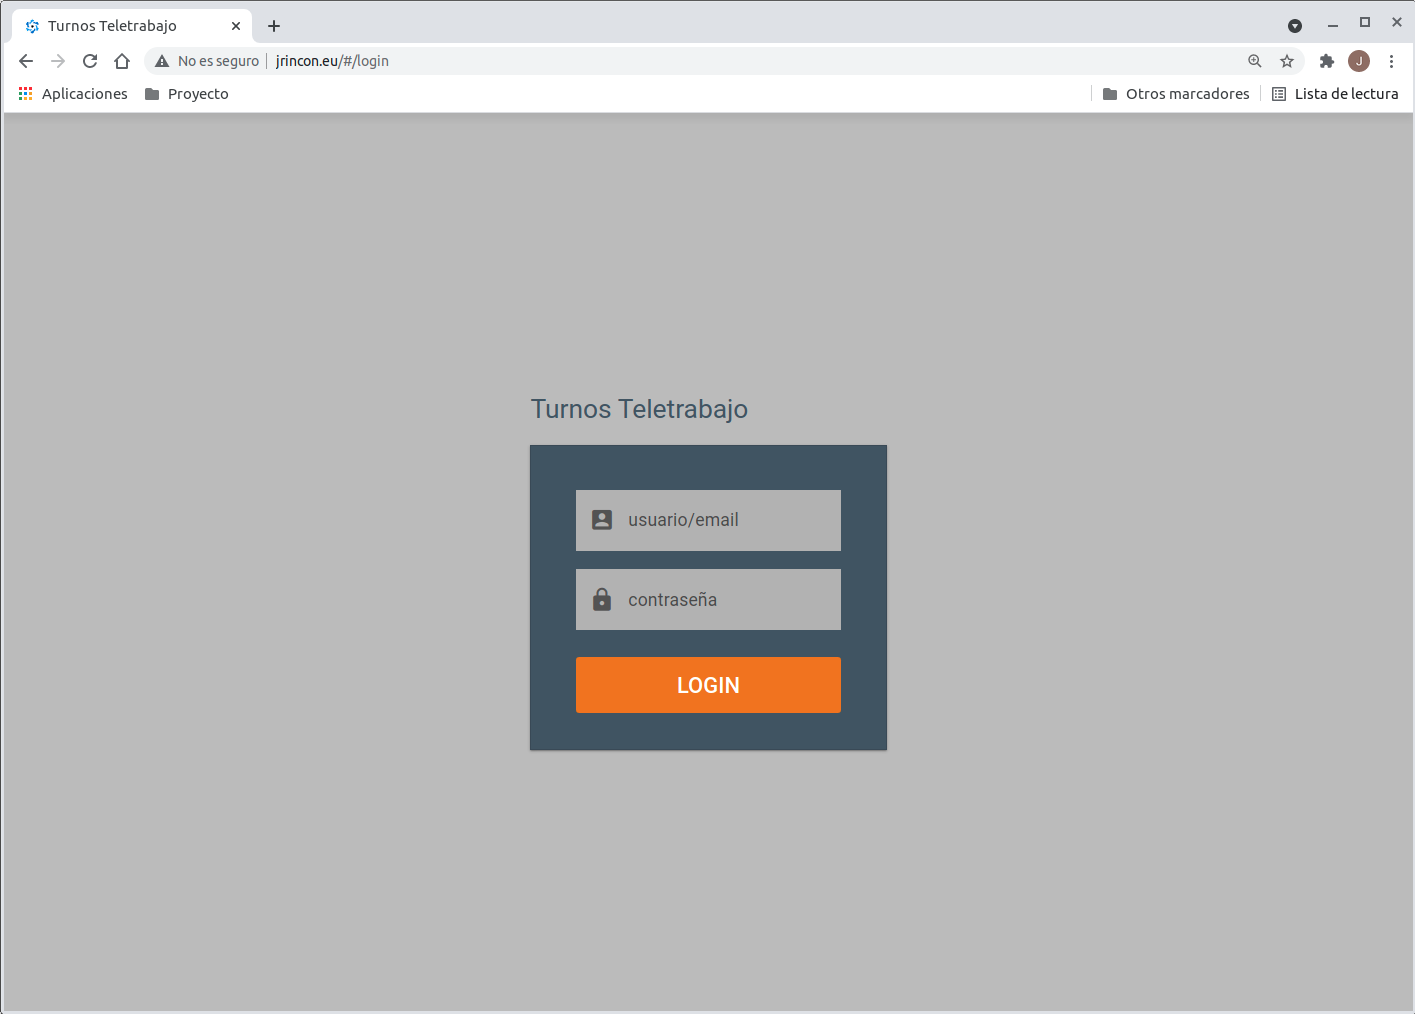
\includegraphics[width=0.49\textwidth]{img/loginweb.png}
  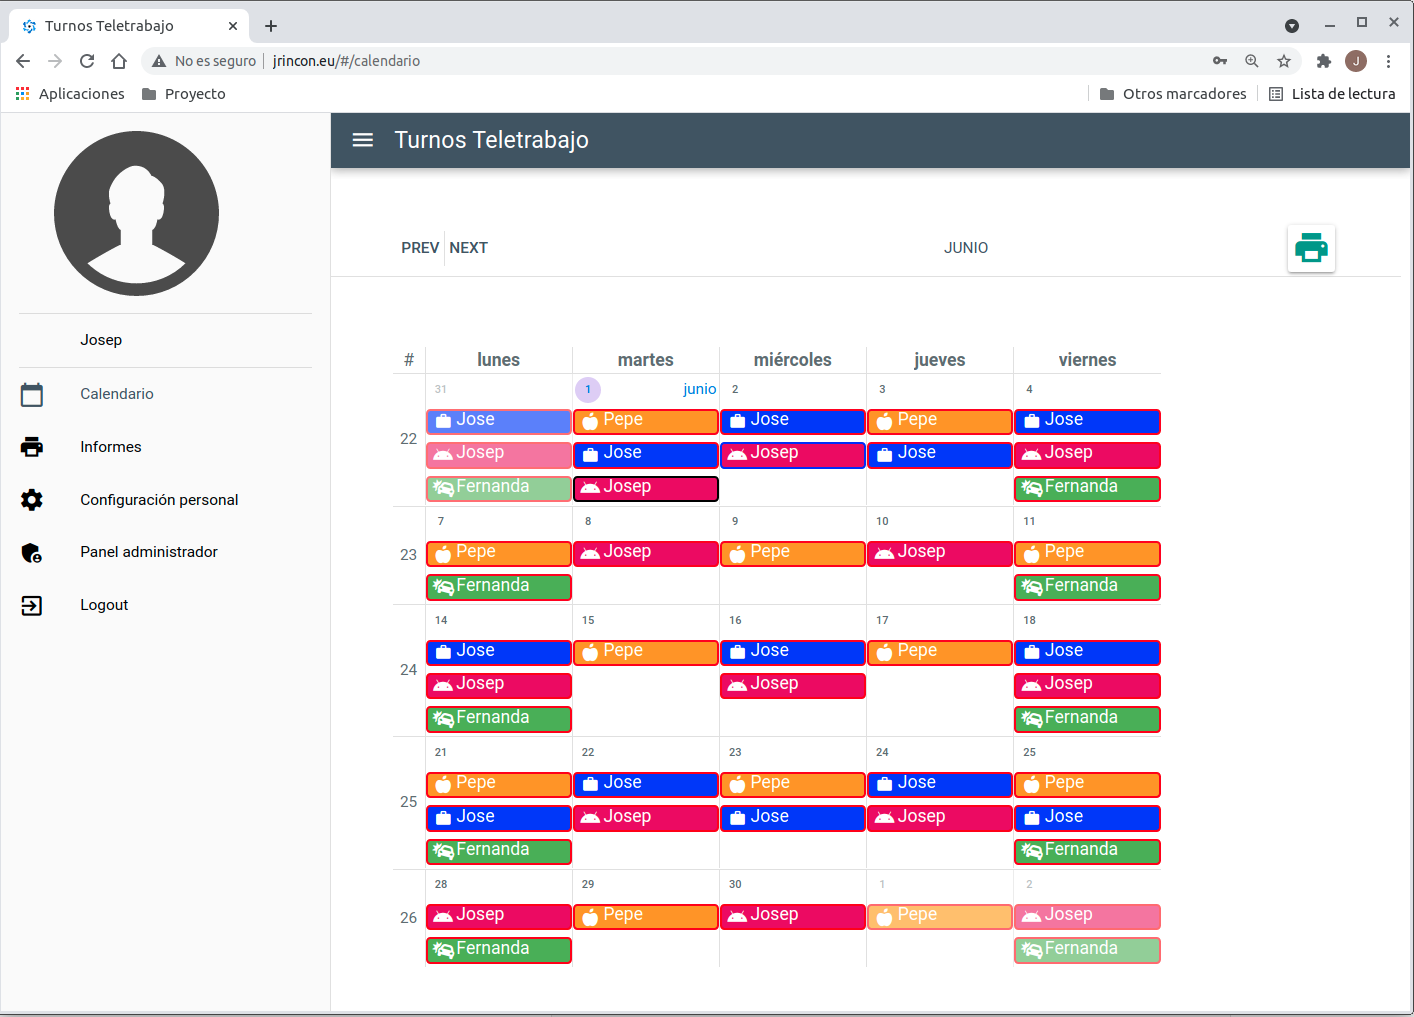
\includegraphics[width=0.49\textwidth]{img/calendarioweb.png}
  \caption{Página de login VS Página ya identificado}
  \label{fig:loginvscalendario}
\end{figure}

Para la autenticación se usa, aparte de Axios y de JWT, Vuex para compartir la información de la autenticación, mutaciones para modificar el estado del usuario. 
\begin{lstlisting}[style=ES6, caption={Estados Vuex autenticación}]
  export const AUTH_REQUEST = state => {
    state.status = "loading";
  };
  export const AUTH_SUCCESS = state => {
    state.status = "success";
  };
  export const AUTH_ERROR = state => {
    state.status = "error";
  };
  export const AUTH_LOGOUT = state => {
    state.status = "logout";
  };
\end{lstlisting}

También se ha usado localstorage para almacenar los detalles del usuario, el token JWT, para así poder guardar la sesión. 
\clearpage
A continuación, un fragmento del código de login y logout:

\begin{lstlisting}[style=ES6, caption={Dispatch de una acción Vuex en el login}]
  import { api } from "boot/axios";
  export function AUTH_REQUEST({ commit, dispatch }, user) {
    return new Promise((resolve, reject) => {
      // The Promise used for router redirect in login
      commit("AUTH_REQUEST");
      api
        .post("/api/auth/signin", user)
        .then(resp => {
          // store the token in localstorage
          localStorage.setItem("user-token", resp.data.accessToken); 
          //... Omitimos el resto de items a localstorage
          commit("AUTH_SUCCESS");
          // you have your token, now log in your user :)
          //dispatch("USER_REQUEST");
          resolve(resp);
        })
        .catch(err => {
          commit("AUTH_ERROR", err);
      // if the request fails, remove any possible user token if possible
          localStorage.removeItem("user-token"); 
          reject(err);
        });
    });
  }  
  export function AUTH_LOGOUT({ commit, dispatch }) {
    return new Promise((resolve, reject) => {
      // The Promise used for router redirect in login
      commit("AUTH_LOGOUT");
      localStorage.removeItem("user-token");
      resolve();
    });
  }
\end{lstlisting}

El menú lateral se ha creado como componente, renderizando los puntos de menú de forma condicional al rol que se ha obtenido en el login.

\begin{lstlisting}[style=ES6, caption={Renderización condicional de punto de menú Admin}]
  <q-item to="/admin" exact v-if="rol === "admin">
  <q-item-section avatar>
    <q-icon name="admin_panel_settings" />
  </q-item-section>

  <q-item-section>
    Panel administrador
  </q-item-section>
</q-item>
\end{lstlisting}

Al existir 3 niveles de acceso, actualmente se obtienen 3 posibles renderizados, si fuera necesario ampliar los niveles de acceso, por ejemplo, un rol para el director de personal, se podrían seguir añadiendo puntos de menú comprobando el rol.

\begin{figure}[ht!] % [h!]
  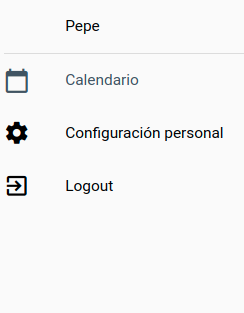
\includegraphics[width=0.33\textwidth]{img/menubase.png}
  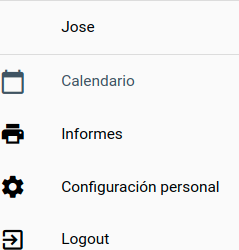
\includegraphics[width=0.33\textwidth]{img/menuresp.png}
  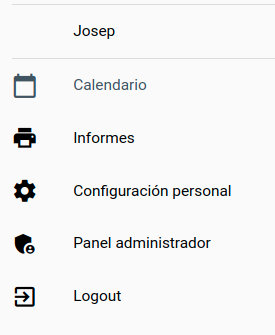
\includegraphics[width=0.33\textwidth]{img/menuadmin.png}
  \caption{Distintas opciones dependiendo del rol}
  \label{fig:menurol}
\end{figure}

En la personalización se ha utilizado el componente q-icon-picker, que nos da acceso a los iconos integrados con quasar, para poder usarlos, en este caso, en la personalización de los usuarios. 

También se ha usado el componente q-color, para dotar de una paleta de colores al usuario, asegurándonos que no se repite ninguno al filtrar la lista de colores que se muestra. 
La paleta de colores permitía elegir cualquier color tanto RGB como hexadecimal, se decidió limitar la cantidad de colores para que 2 personas del mismo departamento no pudieran elegir colores que no se pudieran distinguir, por ejemplo, los rosas rgb(255,0,254) y rgb(255,0,255).

\begin{figure}[ht!] % [h!]
  \centering
  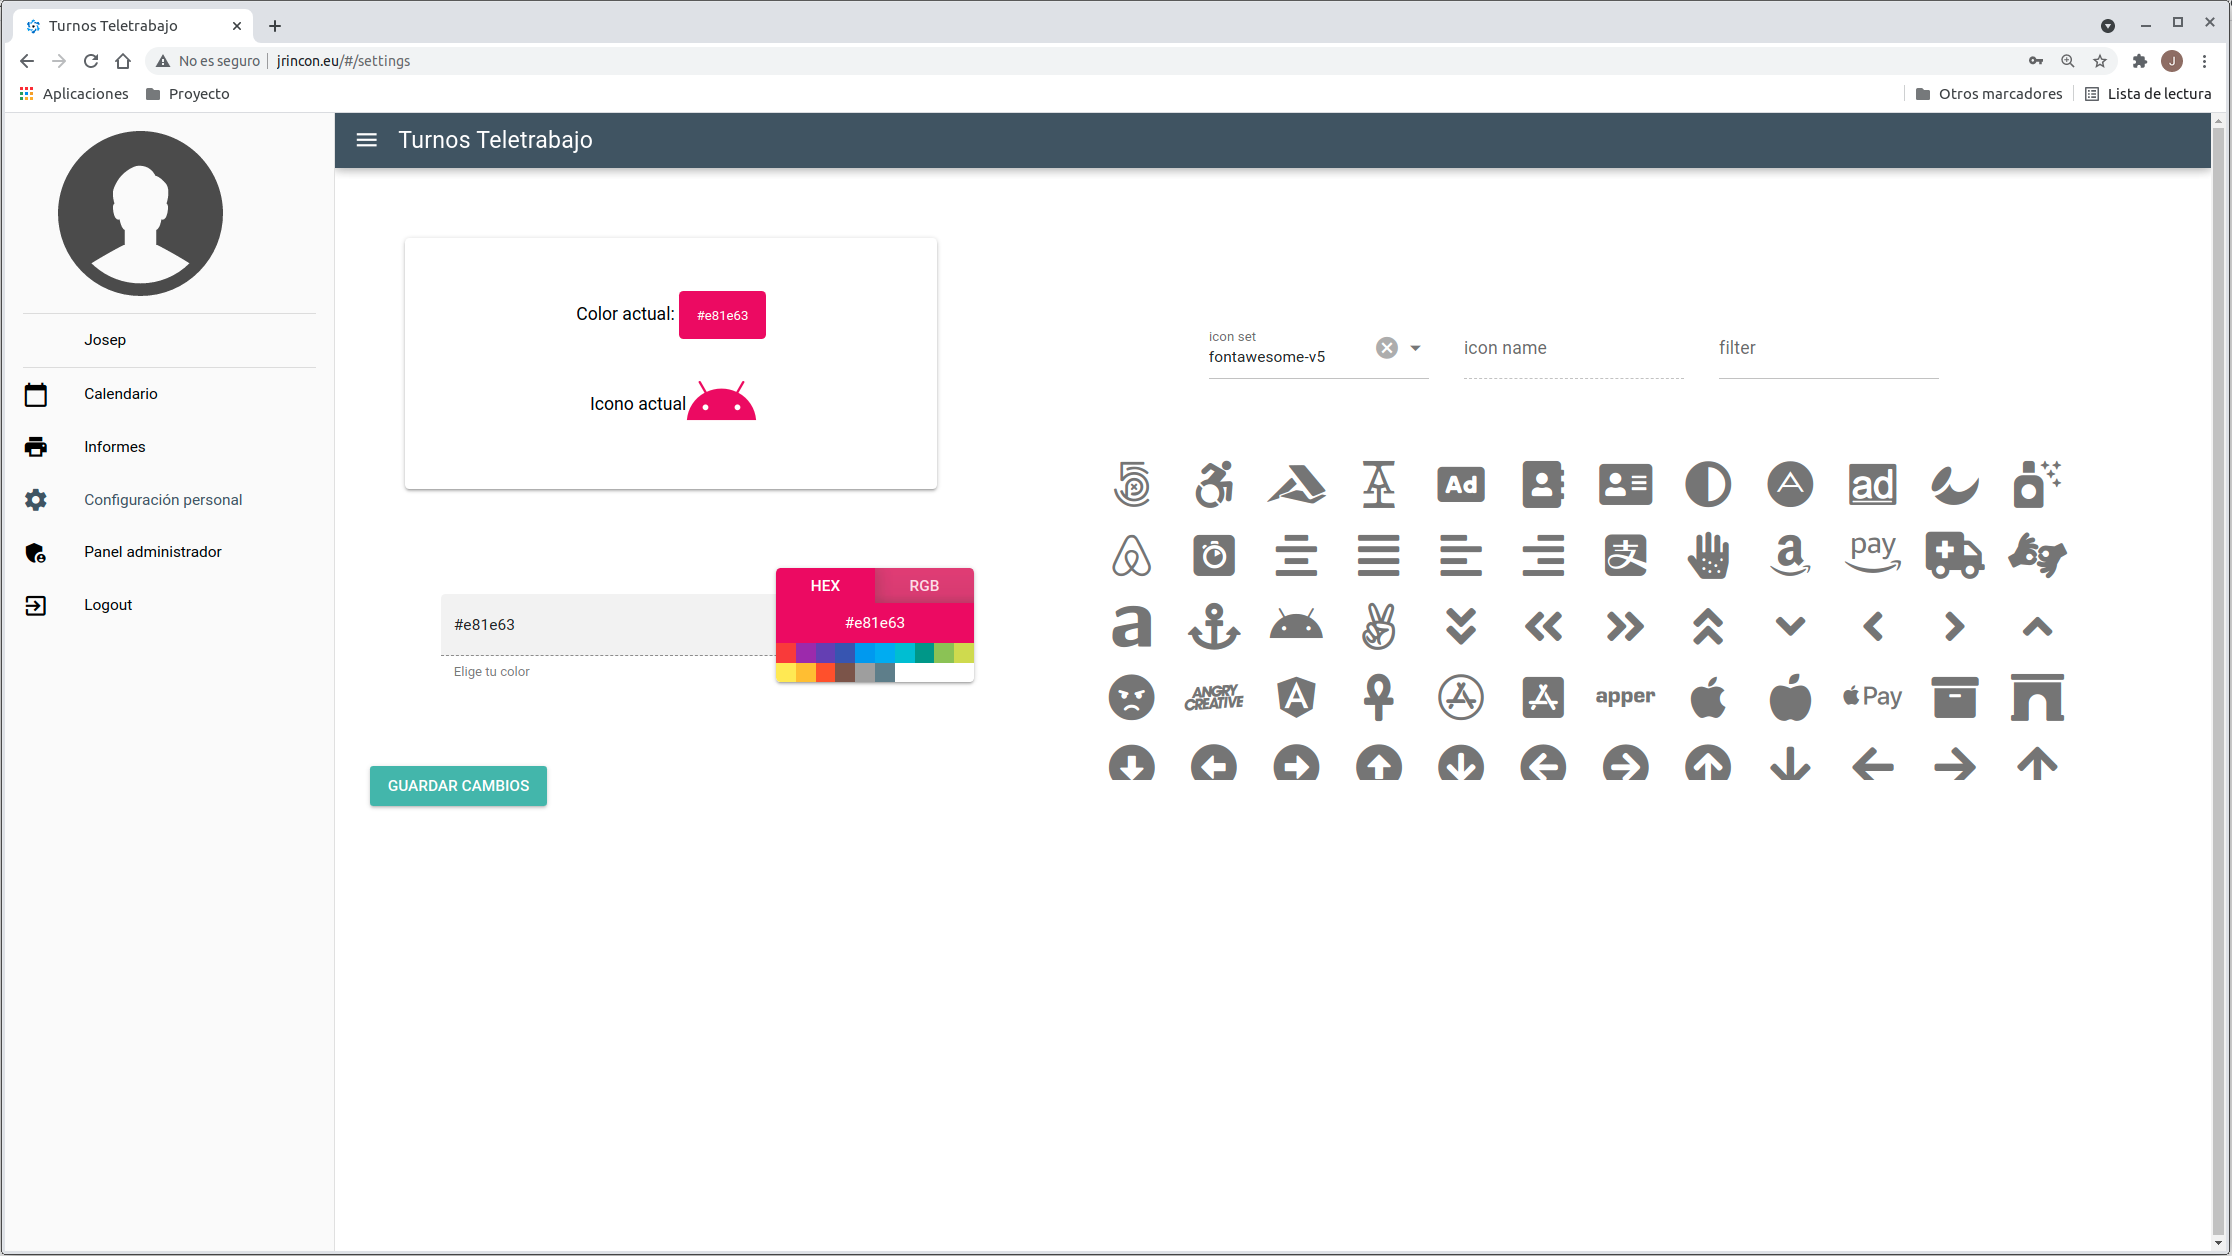
\includegraphics[width=0.90\textwidth]{img/opcionesweb.png}
  \caption{Menú de personalización del icono}
  \label{fig:menupersonalizacion}
\end{figure}

El responsable de departamento tiene a su disposición estadísticas de día x usuario, usuario x día, total de días que ha trabajado un usuario y el porcentaje de presencializadad por día. 

Para la generación de las gráficas, se ha utlizado Vue-ApexCharts, que es un componente generado en base a la librería Apexcharts, librería que permite generar gráficas en múltiples lenguajes de programación.
\newpage

\begin{figure}[ht!] % [h!]
  \centering
  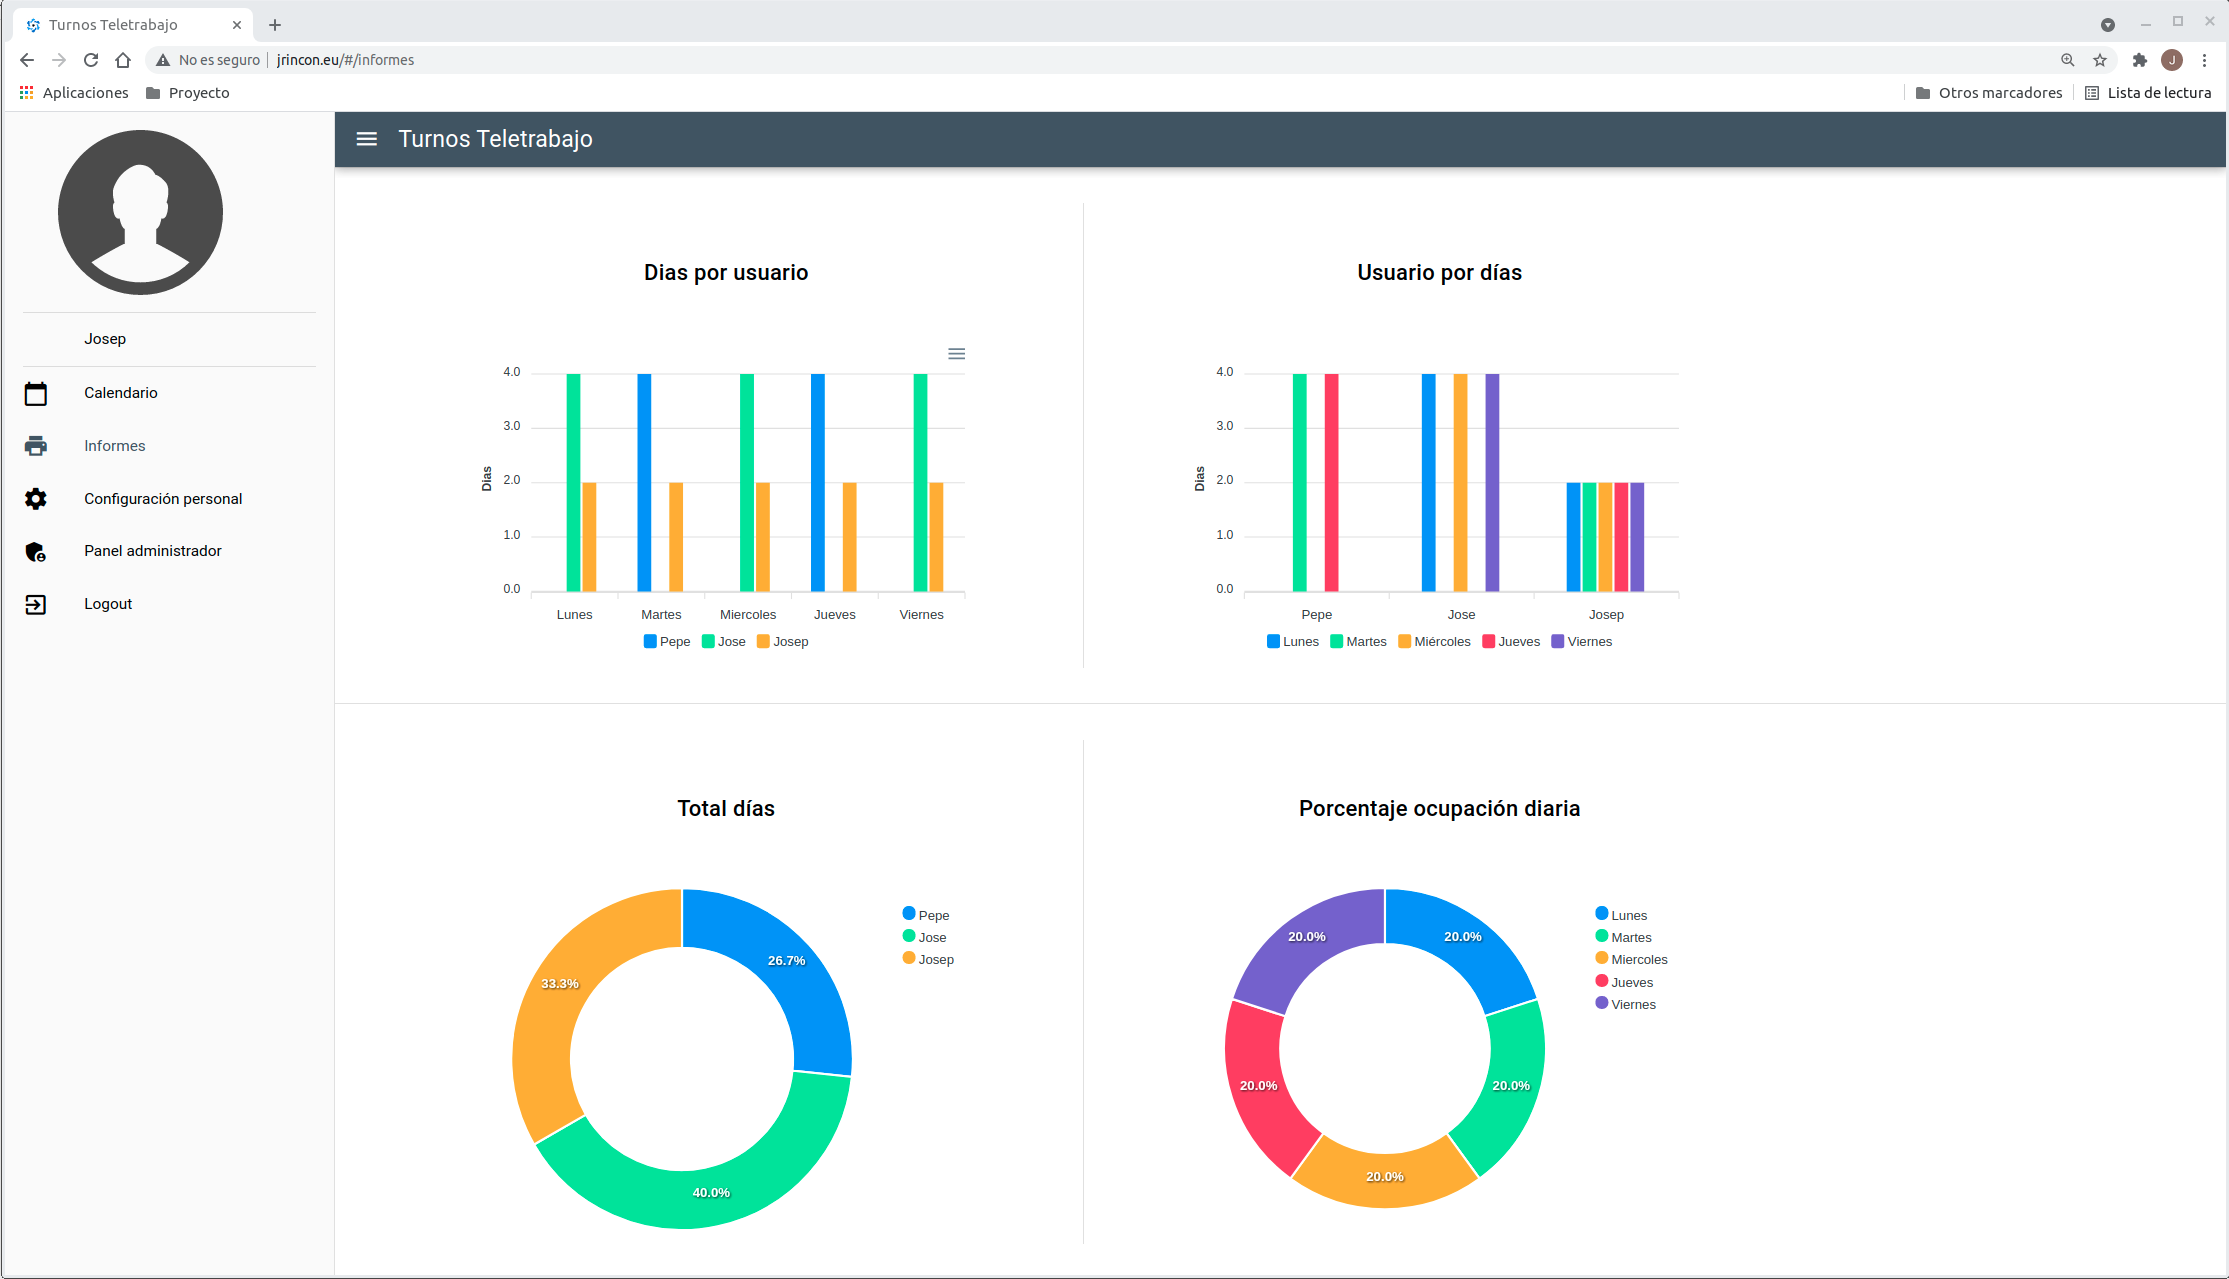
\includegraphics[width=0.90\textwidth]{img/informes.png}
  \caption{Menú de informes}
  \label{fig:menuinformes}
\end{figure}

Se ha creado una tabla para gestionar los usuarios, si bien en entornos empresariales no suele ser común realizar el alta de usuarios a mano (ni el alta automática), se ha dejado para una futura versión el integrar OAUTH  y SSPI.
Para generar la tabla, se ha usado el componente qtable, creando el cuerpo de la tabla a mano para poder insertar componentes q-popup-edit para modificar los datos. 

Finalmente se ha desestimado la grabación inmediata al editar un campo, requiriendo que se valide la información mediante el botón Actualizar.

\begin{figure}[ht!] % [h!]
  \centering
  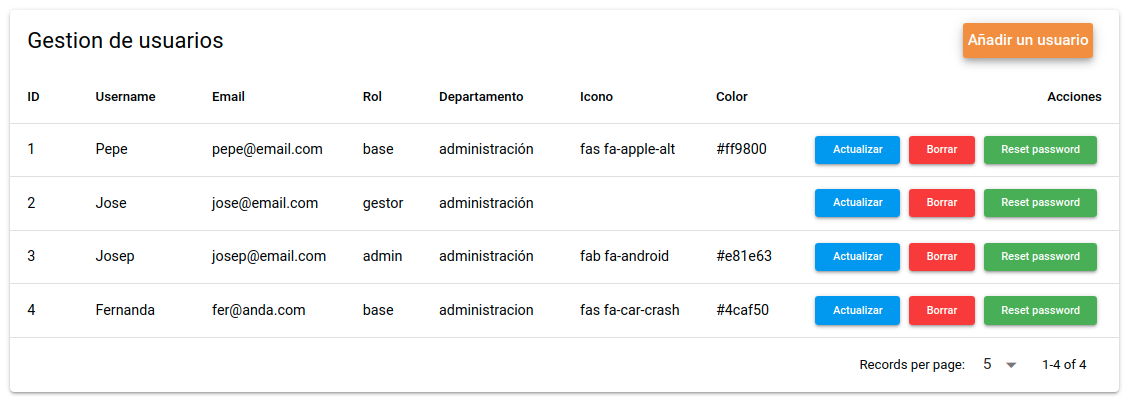
\includegraphics[width=0.90\textwidth]{img/gestionusuarioweb.png}
  \caption{Tabla de gestión de usuarios}
  \label{fig:gestionusuarios}
\end{figure}

% Despliegue
\chapter{Despliegue}

El despliegue se ha realizado mediante docker-compose (compose file en \url{https://github.com/jrinconm/docker-turnos}) en una instancia de Google Cloud, expuesto a Internet en la siguiente dirección:
\url{http://jrincon.eu}. El usuario para entrar en la aplicación es Pepe, Jose, Josep dependiendo el nivel de acceso, y en los tres casos la contraseña es azul.

\section{Configuración de la instancia}
En primer lugar, tenemos que entrar en \href{https://console.cloud.google.com/}{Google Cloud} con una cuenta de Google, nos pedirá que indiquemos el país de procedencia, y que aceptemos las condiciones del servicio.
Opcionalmente, también podemos elegir si queremos recibir más comunicaciones por parte de Google.

Para desplegar la aplicación a través de docker-compose, debemos crear una instancia de una máquina virtual, por lo que en el menú lateral seleccionamos "Compute Engine", que por defecto nos envía a instancias de VM.
El sistema nos pide que creemos un proyecto (si no tenemos ningún otro) y lo nombremos, en mi caso se ha elegido Turnos de Teletrabajo.

En este momento, si no tenemos saldo en Google Cloud, nos pide que rellenemos los datos personales (y los de una tarjeta bancaria) para crear una cuenta, y nos ofrece crédito para trabajar durante 90 días. 
Hemos elegido realizar la prueba de 90 días, ya que se comprometen a no cargar nada en la tarjeta sin nuestro consentimiento.

Una vez que hemos creado el proyecto, nos da paso a crear una instancia de máquina virtual para nuestro proyecto. 
Nos pide nombre de la instancia (se ha dejado el que aparece por defecto), la región y zona dentro de la región donde están ubicados los recursos y la configuración de máquina.

La configuración de la máquina ha sido la más sencilla, e2-micro, con 2 virtual cores y 1 Gb de memoria, tal y conforme indica Google en su documentación, es el ideal para ejecutar aplicaciones pequeñas que no necesitan muchos recursos.

\begin{figure}[h!] % [h!]
  \centering
   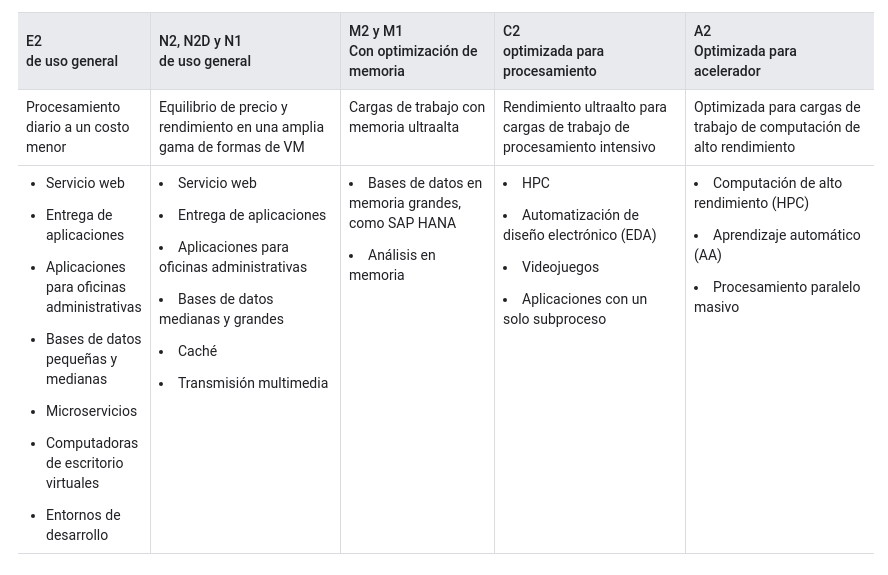
\includegraphics[width=0.90\textwidth]{img/cargas de trabajo.png}
   \caption{Tipos de máquinas según su uso}
   \label{fig:cargas}
 \end{figure}

 En la selección, es necesario elegir abrir el puerto http, para la aplicación web. Así mismo, es necesario el acceso a la API, por lo tanto, tendremos que abrir en el firewall el puerto 8080. 
 Momentáneamente es necesario abrir el puerto 8000 para phpmyadmin, para crear e importar la base de datos, si no queremos hacerlo por la línea de comandos.

 Actualmente, está consumiendo un 9\% - 15\% de la cpu, y al estar casi uso (actualmente testing), prácticamente no escribe en disco ni genera datos por la red.

 \begin{figure}[H] % [h!]
  \centering
   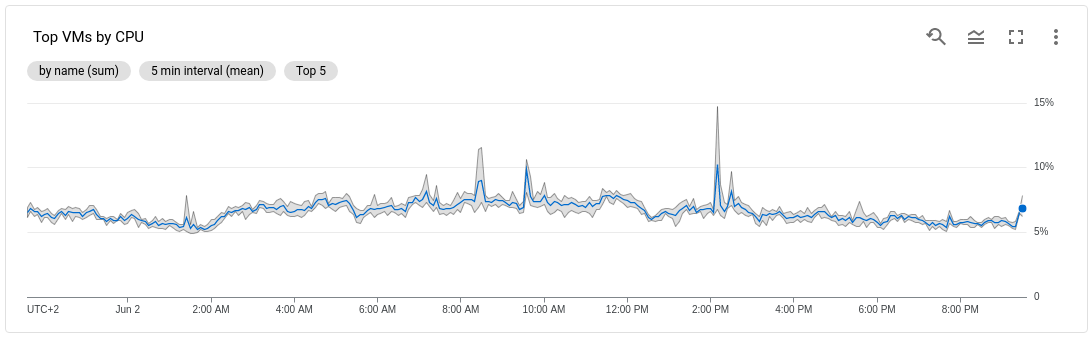
\includegraphics[width=0.90\textwidth]{img/usocpu.png}
   \caption{Carga de la cpu durante un día}
   \label{fig:cargaweb}
 \end{figure}

 \begin{figure}[H] % [h!]
  \centering
   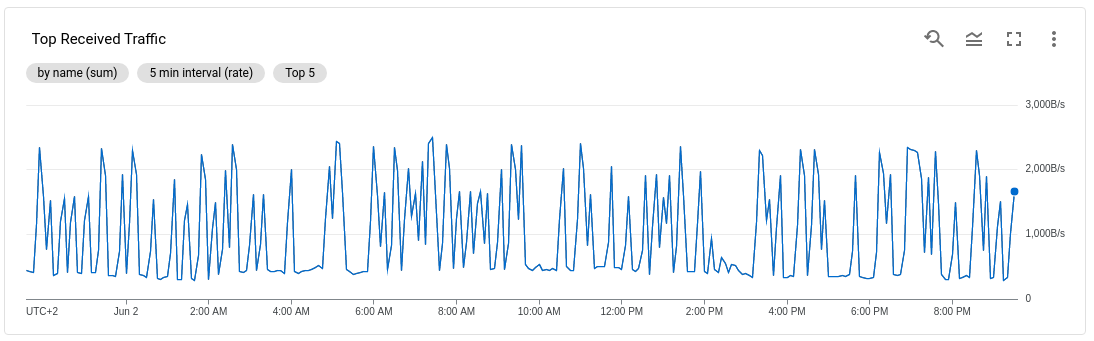
\includegraphics[width=0.90\textwidth]{img/usonet.png}
   \caption{Ancho de banda consumido durante un día}
   \label{fig:cargalanweb}
 \end{figure}

 \begin{figure}[H] % [h!]
  \centering
   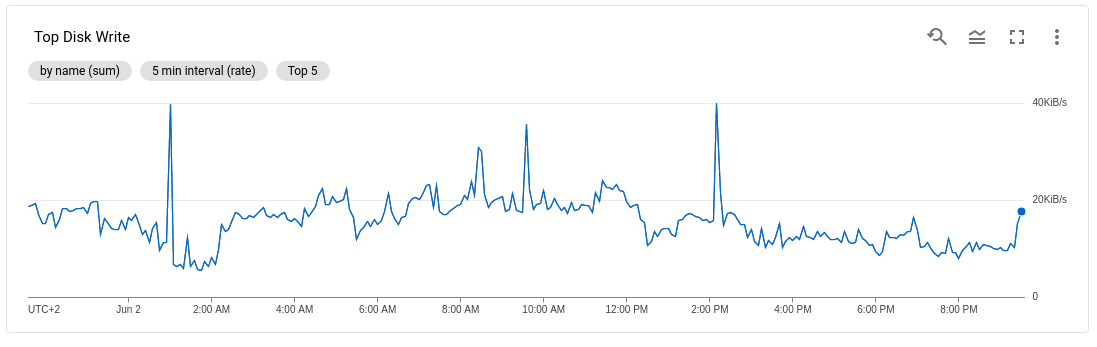
\includegraphics[width=0.90\textwidth]{img/usodisco.png}
   \caption{Tasa de escritura a disco durante un día}
   \label{fig:cargawhdweb}
 \end{figure}

 \begin{figure}[H] % [h!]
  \centering
   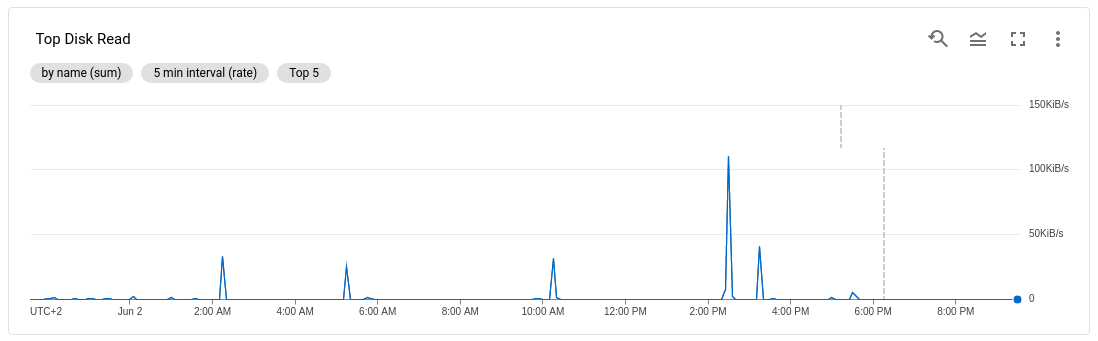
\includegraphics[width=0.90\textwidth]{img/usodiscoread.png}
   \caption{Tasa de lectura de disco durante un día}
   \label{fig:cargarhdweb}
 \end{figure}

\section{Instalación de los archivos}

En el momento que está creada la instancia, y corriendo, nos podemos conectar a ella a través de ssh. Para ello, sólo tenemos que pulsar el cuadro que pone ssh y se nos abre un navegador con una consola ssh del equipo.

En este punto, la instalación es igual que en un servidor dedicado o físico dentro de nuestra infraestructura. En la consola, descargamos de github el docker-compose del proyecto \href{https://github.com/jrinconm/docker-turnos/}{docker-turnos}.
Por ejemplo, clonando el repositorio, o directamente con wget. 

Una vez descargado, al no estar instalado docker-compose, lo vamos a ejecutar dentro de un contenedor a su vez también:

\begin{lstlisting}[language=bash, caption={Comando docker para lanzar docker-compose}]
docker run --rm  -v /var/run/docker.sock:/var/run/docker.sock -v "$PWD:$PWD"   -w="$PWD"  docker/compose:1.24.0 up \d
\end{lstlisting}
Este comando nos levantara tanto los contenedores de la aplicación, como un contenedor puntual de phpmyadmin para que podamos crear la base de datos, restaurar un backup, o modificar lo que creamos conveniente.

Una vez levantado todo el sistema, sólo nos falta comprobar en el panel, cual es la dirección ip externa, para comprobar que se ha levantado correctamente nuestra aplicación. Esta dirección se puede comprobar directamente en la instancia de la máquina virtual.

\begin{figure}[H] % [h!]
  \centering
   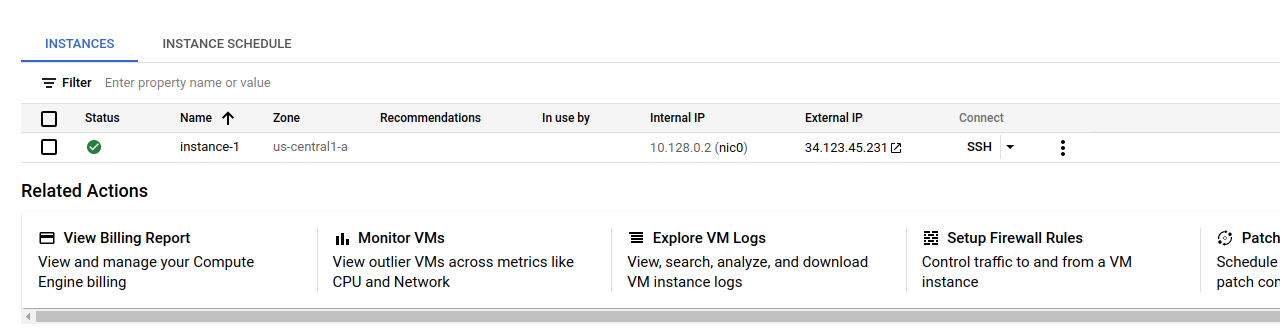
\includegraphics[width=0.90\textwidth]{img/ipexterna.png}
   \caption{Ip externa 34.123.45.231}
   \label{fig:ipexterna}
 \end{figure}

Si queremos eliminar los contenedores, primero debemos pararlos de forma individual, o utilizamos el mismo contenedor con docker-compose que hemos usado anteriormente:

\begin{lstlisting}[language=bash, caption={Comando docker para parar docker-compose}]
docker run --rm  -v /var/run/docker.sock:/var/run/docker.sock -v "$PWD:$PWD"   -w="$PWD"  docker/compose:1.24.0 down
\end{lstlisting}

Para eliminar las imágenes que se han descargado del repositorio jrincon, pero no la de mariadb ni las que tiene google cloud asociadas a la instancia, podemos ejecutar el siguiente comando:

\begin{lstlisting}[language=bash, caption={Borrado de imágenes con el texto jrincon}]
  docker images|grep jrincon|awk {'print $3'}|xargs docker image rm
\end{lstlisting}

En el caso que necesitemos modificar uno de los contenedores, por ejemplo, para cambiar las contraseñas, sólo tenemos que clonar el repositorio, realizar la edición y dentro del directorio donde está el dockerfile, ejecutar:

\begin{lstlisting}[language=bash, caption={Comando docker para construir una imagen}]
  docker build  --pull -f "Dockerfile"  "."
\end{lstlisting}

Lo podemos compilar y nombrar al mismo tiempo, con el parámetro -t para ponerle el tag a la imagen compilada. Una vez compilada, podemos hacerle un push para subir la imagen a nuestro repositorio docker.

Para nuestra referencia, en 7 días el crédito no se ha consumido, desde la creación inicial de la instancia:

\begin{figure}[h!] % [h!]
  \centering
   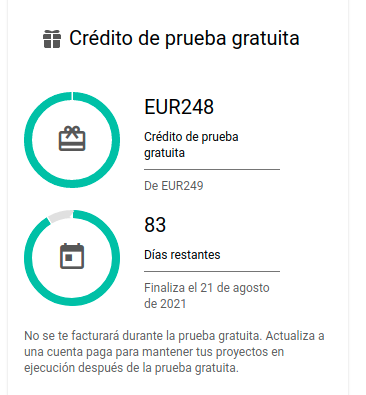
\includegraphics[width=0.20\textwidth]{img/Credito.png}
   \caption{Crédito restante en Google Cloud}
   \label{fig:creditogoogle}
 \end{figure}

\chapter{Herramientas de apoyo}

Se ha usado Visual Studio Code como IDE, se ha configurado un workspace con los diferentes subproyectos, y se han instalado las siguientes extensiones:
\begin{itemize}
  \item Docker. Permite crear y gestionar los contenedores.
  \item ESlint. Integra el linter ESlint en VSCode.
  \item Git History. Permite comparar commits y ramas.
  \item GitLens. Permite hacer un diff de los cambios frente el ultimo commit, entre muchas más opciones.
  \item LaTeX Workshop. Previsualiza y compila código LaTeX.
  \item Prettier. Formateador de código usado.
  \item Vetur. Añade intellisense Vue.
\end{itemize}

Se ha usado Sonarqube para analizar la calidad del código, me ha ayudado a hacer más seguro el código, eliminando posibles puntos de fallo, así como limpiar código duplicado.

Actualmente, Sonarqube le da la máxima calificación a mi código, tanto en bugs, como en vulnerabilidades, y en el caso del frontend de líneas duplicadas.

\begin{figure}[h!] % [h!]
  \centering
   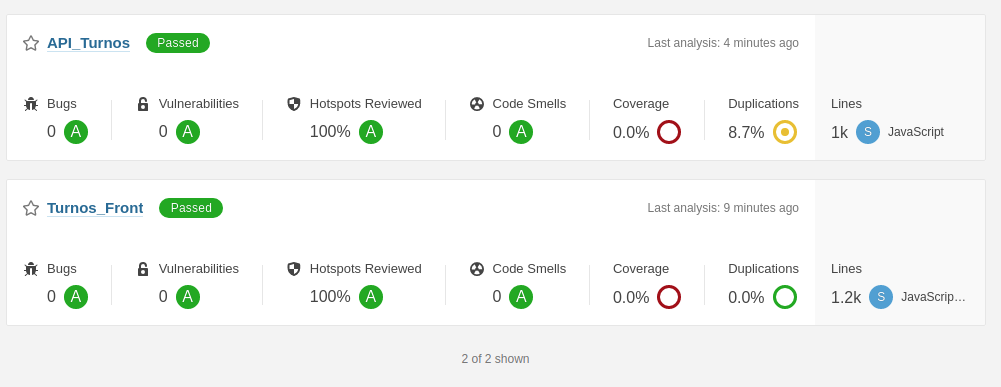
\includegraphics[width=0.90\textwidth]{img/estadosonar.png}
   \caption{Análisis del código por Sonarqube}
   \label{fig:estadosonar}
 \end{figure}
\clearpage
Como curiosidad, integra una utilidad para ver como una ciudad el código, siendo los edificios los ficheros, las manzanas los subdirectorios, de esta forma, de un sólo vistazo, se puede ver qué ficheros son los que contienen más líneas de código, por si es necesario refactorizar.

\begin{figure}[h!] % [h!]
  \centering
   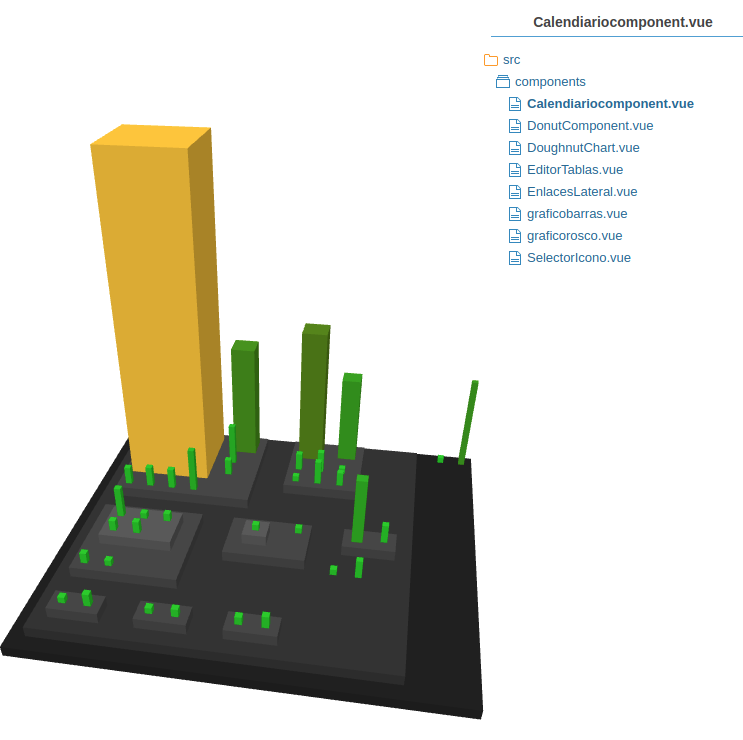
\includegraphics[width=0.50\textwidth]{img/calendarioSonarqube.png}
   \caption{Fichero calendario.vue en vista 3d}
   \label{fig:calendariosonar}
 \end{figure}

También se ha usado git para el control de versiones, siendo Github la plataforma usada. Dentro de esta plataforma, tenemos un componente CI/CD que lo han llamado Github Actions, que he empleado para compilar el código látex según iba realizando los commits.

Una vez compilado el documento, lo dejaba como un artefacto de esa build, comprimido en un zip. 

\begin{lstlisting}[style=ES6, caption={Configuración action github}]
  name: Build LaTeX document
  on: [push]
  jobs:
    build_latex:
      runs-on: ubuntu-latest
      steps:
        - name: Set up Git repository
          uses: actions/checkout@v2
        - name: Compile LaTeX document
          uses: xu-cheng/latex-action@v2
          with:
            root_file: TFGJrincon.tex
        - uses: actions/upload-artifact@v2
          with:
            name: PDF
            path: TFGJrincon.pdf
\end{lstlisting}
\clearpage
Para realizar las pruebas de funcionamiento de la API, se ha usado \href{https://www.postman.com/}{Postman}, creando una colección de consultas para poder repetirlas posteriormente.

A continuación, muestro una consulta en la que se realiza el signin con usuario Pepe y la contraseña azul, obteniendo el jsonwebtoken que se muestra en la imagen.

\begin{figure}[h!] % [h!]
  \centering
   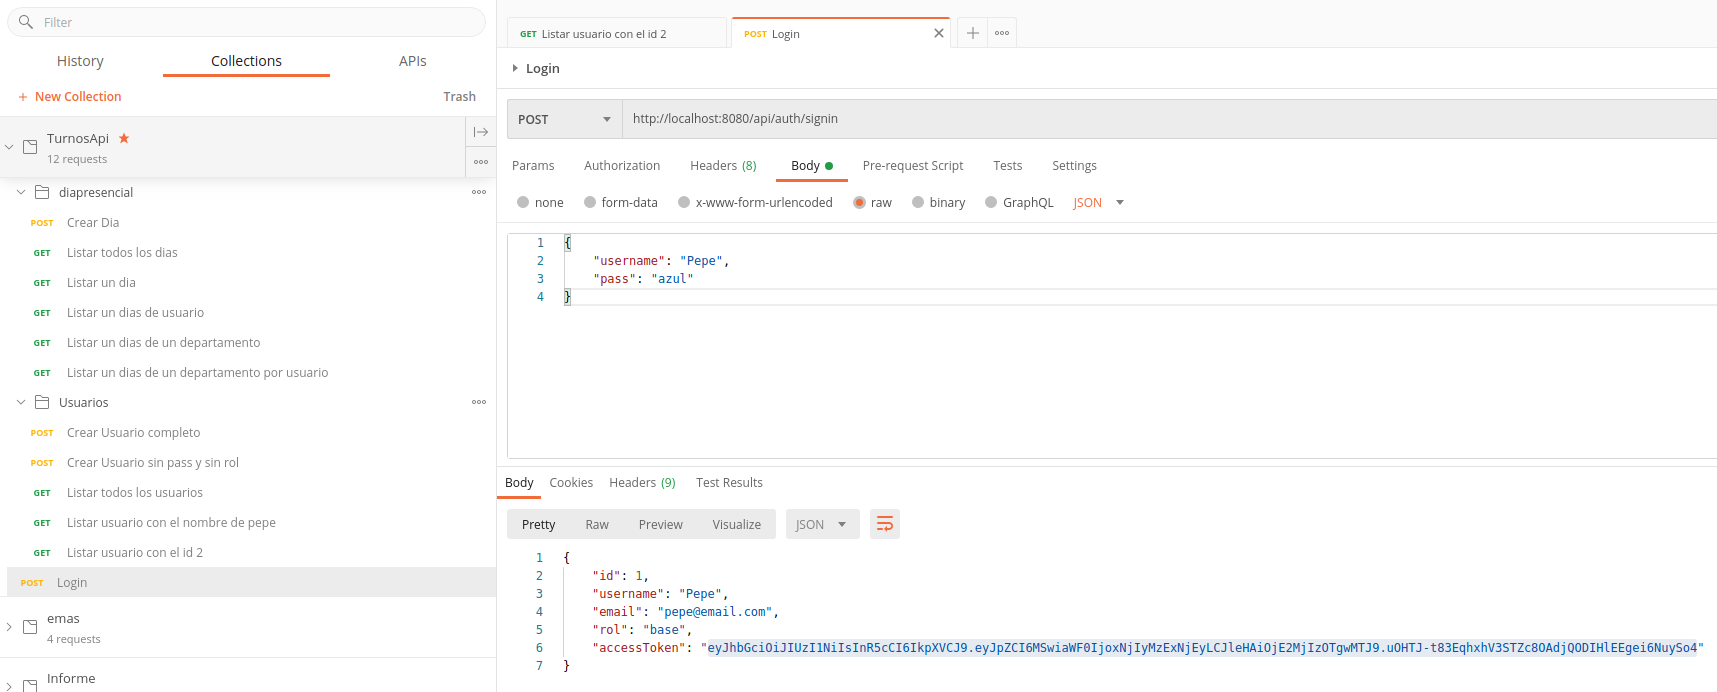
\includegraphics[width=\linewidth]{img/postman.png}
   \caption{Colección consultas postman}
   \label{fig:postman}
 \end{figure}

Se ha elegido Docker y Docker Compose como entorno de virtualización, y en mi perfil del hub están las imágenes compiladas para poder desplegarlas de forma rápida. 

Para la realización de los mockups se ha usado el site \href{https://mockflow.com/app/#Wireframe}{Mockflow}.

En la parte de los diagramas se ha usado el site \href{https://lucid.app/}{Lucid}, que anteriormente se llamaba directamente LucidChart, y Visual Paradigm.

%%%%%%%%%%%%%%%%%%%%%%%%%%%%%%%%%%%%%%%%%%%%%%%%%%%%%%%%%%%%%%%%%%%%%%%%%%%%%%%
%                                 CONCLUSIONS                                 %
%%%%%%%%%%%%%%%%%%%%%%%%%%%%%%%%%%%%%%%%%%%%%%%%%%%%%%%%%%%%%%%%%%%%%%%%%%%%%%%

\chapter{Conclusiones}

La combinación de Node.js con Express y sequelize permite crear una API de una forma simple, que combinado con la velocidad que de maquetación de Quasar, nos permite crear aplicaciones de forma rápida.
Si unimos analizadores de código, como Sonarqube, añadimos a la velocidad de creación, seguridad, limpieza y estabilidad. 
El código lo podemos probar en entorno de pruebas con contenedores docker, que a su vez nos permitirán desplegarlo de forma ágil, tanto en la nube como en nuestra propia infraestructura.

Personalmente, la elección de javascript para el backend, si bien no lo vimos en entorno servidor, creo que ha sido positiva, puesto que me ha permitido conocer el entorno de Node.js. 
No he necesitado aprender a usar el lenguaje, puesto que ya lo conocía, y sólo he tenido que leer a documentación existente para crear una API sólida, que si bien puede ser mejorable, es suficiente para el uso requerido.

También estoy contento con la elección de sequelize, puesto que al modificar la estructura de la base de datos, sólo tuve que modificar las clases que representan las tablas en la base de datos. 
Al cambiar también el nombre de los campos (por ejemplo, cambié RolId por Rol), tuve que modificar alguna función de los controllers que solicitaba expresamente el campo renombrado, pero con sólo buscar el campo y realizar la sustitución fue suficiente.

Posiblemente, si en el primer análisis se hubieran detectado sólo 2 tablas, habría realizado las consultas a mano, descartando el uso de Sequelize, puesto que posiblemente realizar las consultas puntualmente, hubiera sido más rápido.

Para comprobar que la API funcionaba correctamente, he realizado un uso intensivo de Postman, que, una vez configurado con todas las consultas creadas, de una forma muy rápida pude comprobar que devolvía lo esperado.
Me ha sido especialmente útil una vez modificada la base de datos, para comprobar que seguía devolviendo y requiriendo la misma información. 

En la parte cliente, he descubierto la librería ApexCharts para la generación de gráficas, que me ha parecido muy interesante y cómoda de usar, muy configurable. Me ha parecido mucho más sencilla de usar y mejor documentada que chart.js.

Quasar como frontend me pareció muy completo, ya que abarca desde el diseño del interfaz a través de clases de forma similar a bootstrap, hasta componentes muy variados, desde tablas, hasta popups. 

En alguna ocasión he instalado un componente externo, para a los pocos días, darme cuenta que ya tenía incluida de forma nativa un componente con la misma utilidad, por ejemplo Vue Toasted (componente notify de quasar)  y dialog.

Creo que he acertado eligiendo Quasar, según lo he ido usando y descubriendo nuevas opciones, me ha parecido más facil implementar nuevas funciones. 

\section{Mejoras y ampliaciones del programa}

La aplicación actualmente es práctica y funcional, sin embargo, hay múltiples funcionalidades que pueden ampliarla y mejorarla. A continuación, expongo una lista.

\begin{itemize}
  \item Departamentos, subdepartamentos y áreas. Actualmente sólo hay 1 nivel de departamento, en un futuro se podría ampliar a varios niveles, por ejemplo, dentro de logística, podríamos tener compras, almacén, etc.
  \item Documentar la API según la especificación OpenApi e integrar swagger.
  \item Drag and drop de día presencial sobre el de un compañero, para solicitar el cambio de forma automática. 
  \item Creación de un estado "Vacaciones o no disponible" para marcar que una persona no estará presencialmente (ni de forma remota), sin que aparezca en las estadísticas negativamente.
  \item Generar eventos en el calendario del usuario de office 365 (es necesaria una cuenta office 365 y enlazar la cuenta con la aplicación)
  \item Integrar certificados SSL tanto a la API como al cliente.
\end{itemize}



%%%%%%%%%%%%%%%%%%%%%%%%%%%%%%%%%%%%%%%%%%%%%%%%%%%%%%%%%%%%%%%%%%%%%%%%%%%%%%%
%                                BIBLIOGRAFIA                                 %
%%%%%%%%%%%%%%%%%%%%%%%%%%%%%%%%%%%%%%%%%%%%%%%%%%%%%%%%%%%%%%%%%%%%%%%%%%%%%%%

\begin{thebibliography}{10}

\bibitem{WAR}
   Documentación oficial sequelize.
   \newblock Consultado en 
   \url{https://sequelize.org/master}.

\bibitem{WAR}
   Issue del github de sequelize donde está la definición y ejemplos de clases para definir los modelos.
   \newblock Consultado en
   \url{https://github.com/sequelize/sequelize/issues/6524}.

\bibitem{WAR}
   Documentación oficial Quasar.
   \newblock Consultado en 
   \url{https://quasar.dev/start/pick-quasar-flavour}.

\bibitem{WAR}
   Documentación oficial componente QCalendar.
   \newblock Consultado en 
   \url{https://quasarframework.github.io/quasar-ui-qcalendar/docs}.

\bibitem{WAR}
   Documentación oficial Express.
   \newblock Consultado en 
   \url{https://expressjs.com/es/guide/routing.html}.

\bibitem{WAR}
  Documentación oficial Vuex.
   \newblock Consultado en 
   \url{https://next.vuex.vuejs.org/}.

\bibitem{WAR}
   Documentación oficial Vue-ApexChart.
    \newblock Consultado en 
    \url{https://apexcharts.com/docs/vue-charts/}.

\bibitem{WAR}
   Documentación oficial Google Cloud.
    \newblock Consultado en 
    \url{https://cloud.google.com/docs}.

\bibitem{WAR}
   Howto creación de api con Node, Sequelize, Express y mysql.
   \newblock Consultado en
   \url{https://bezkoder.com/node-js-express-sequelize-mysql}.

\bibitem{WAR}
   Howto autenticación Vue con Vuex.
   \newblock Consultado en
   \url{https://www.digitalocean.com/community/tutorials/handling-authentication-in-vue-using-vuex}.

   \bibitem{WAR}
   Plantillas Latex TFG etsinf.
   \newblock Consultado en
   \url{https://www.inf.upv.es/www/etsinf/es/plantilla-tfg/}.

   

\end{thebibliography}
\cleardoublepage

%%%%%%%%%%%%%%%%%%%%%%%%%%%%%%%%%%%%%%%%%%%%%%%%%%%%%%%%%%%%%%%%%%%%%%%%%%%%%%%
%                           APÈNDIXS  (Si n'hi ha!)                           %
%%%%%%%%%%%%%%%%%%%%%%%%%%%%%%%%%%%%%%%%%%%%%%%%%%%%%%%%%%%%%%%%%%%%%%%%%%%%%%%



%%%%%%%%%%%%%%%%%%%%%%%%%%%%%%%%%%%%%%%%%%%%%%%%%%%%%%%%%%%%%%%%%%%%%%%%%%%%%%%
%                         LA CONFIGURACIO DEL SISTEMA                         %
%%%%%%%%%%%%%%%%%%%%%%%%%%%%%%%%%%%%%%%%%%%%%%%%%%%%%%%%%%%%%%%%%%%%%%%%%%%%%%%





%%%%%%%%%%%%%%%%%%%%%%%%%%%%%%%%%%%%%%%%%%%%%%%%%%%%%%%%%%%%%%%%%%%%%%%%%%%%%%%
%                              FI DEL DOCUMENT                                %
%%%%%%%%%%%%%%%%%%%%%%%%%%%%%%%%%%%%%%%%%%%%%%%%%%%%%%%%%%%%%%%%%%%%%%%%%%%%%%%

\end{document}
